%\section{SECCIÓN: SIMULACIÓN EN LTSPICE}

\subsubsection{Fundamentación de Directivas SPICE Empleadas}
Para la caracterización del amplificador multietapa se empleó el entorno de simulación \textbf{LTspice®}. Con el objetivo de automatizar y estandarizar la obtención de parámetros eléctricos, se utilizaron las siguientes directivas fundamentales de forma genérica:

\begin{itemize}
    \item \texttt{.op} \textbf{(Punto de Operación DC):} Evalúa las tensiones continuas de nodo y corrientes de rama sin señal aplicada, permitiendo verificar la zona de trabajo activa de los semiconductores y su disipación de potencia estática.
    \item \texttt{.ac <type> <n> <fstart> <fstop>} \textbf{(Análisis de Pequeña Señal AC):} Realiza un barrido frecuencial de pequeña señal para obtener la respuesta en frecuencia (Diagrama de Bode), ganancias de tensión e impedancias complejas de entrada y salida ($Z_{in}$, $Z_{out}$).
    \item \texttt{.tran <tstep> <tstop>} \textbf{(Análisis Temporal de Transitorios):} Simula la respuesta temporal dinámica del circuito en el dominio del tiempo frente a señales senoidales para evaluar la forma de onda, excursiones pico a pico y simetría de salida.
    \item \texttt{.noise V(node) <src> <type> <n> <fstart> <fstop>} \textbf{(Análisis de Ruido):} Calcula la Densidad Espectral de Potencia (PSD) de ruido térmico y de disparo referida a la salida o entrada del circuito.
    \item \texttt{.four <freq> V(out)} \textbf{(Análisis de Fourier):} Procesa la señal temporal del análisis \texttt{.tran} aplicando la Transformada Rápida de Fourier (FFT) para calcular la Distorsión Armónica Total (THD) evaluando hasta el 9no armónico respecto a la componente fundamental.
    \item \texttt{.step param <var> list <val1> <val2>...} \textbf{(Análisis Paramétrico):} Ejecuta simulaciones iterativas variando parámetros como la amplitud de entrada ($A_{in}$), la impedancia de carga ($R_L$) o las tensiones de alimentación ($V_{CC}$) para determinar analíticamente los límites de operabilidad y estabilidad lineal observando la deformación o recorte de la señal en la salida.
    \item \texttt{.meas <type> <name>  FIND <expr> AT/WHEN <cond>} \textbf{(Mediciones Condicionales con FIND):} Permite extraer valores exactos de magnitudes eléctricas (tensiones, corrientes, impedancias o desfases) evaluados en puntos o frecuencias específicas (por ejemplo, evaluar la ganancia o impedancia exactamente a $1\,\text{kHz}$ mediante \texttt{.meas AC Zin FIND Mag(V(in)/I(Vin)) AT=1k}).
\end{itemize}
\subsubsection{Modelos SPICE de Transistores Empleados}
Para garantizar una simulación acorde a los transistores reales utilizados, se incorporaron al esquema las siguientes directivas de modelo de parámetros SPICE para los semiconductores NPN y PNP:

\begin{lstlisting}
* Modelo TIP122 
.model Q5 PNP (IS=1e-11 BF=1000 VAF=100 IKF=3 ISE=1e-10 NE=2 BR=4 VAR=20 RB=10 RC=0.1 CJE=1.2e-9 CJC=2.5e-10 VCEO=100 ICN=5)

* Modelo BD139
.model Q2 NPN (IS=2.39e-13 BF=200 VAF=100 IKF=0.8 ISE=1e-14 NE=1.5 BR=3 VAR=20 RB=1.5 RC=0.15 CJE=2e-10 CJC=8e-11 VCEO=80 ICN=1.5)

* Modelo BC546
.model Q1 NPN (IS=1.8e-14 BF=400 VAF=100 IKF=0.15 ISE=5e-15 NE=1.25 BR=5 VAR=20 RB=20 RC=0.6 CJE=1.3e-11 CJC=4.5e-12 VCEO=65 ICN=0.1)

* Modelo BC546
.model Q3 NPN (IS=1.8e-14 BF=400 VAF=100 IKF=0.15 ISE=5e-15 NE=1.25 BR=5 VAR=20 RB=20 RC=0.6 CJE=1.3e-11 CJC=4.5e-12 VCEO=65 ICN=0.1)
\end{lstlisting}
% =========================================================================
% APARTADO 1: GLOBAL
% =========================================================================
\subsubsection{Análisis Global del Amplificador (Simulación Integral)}

%\subsection*{Prueba y Caracterización General del Sistema Completo}
En esta sección se consolida la evaluación del amplificador de 3 etapas interconectado en cascada cargado nominalmente con $R_L = 8\,\Omega$ (\cref{fig:circuito_global}).

\begin{figure}[H]
    \centering
    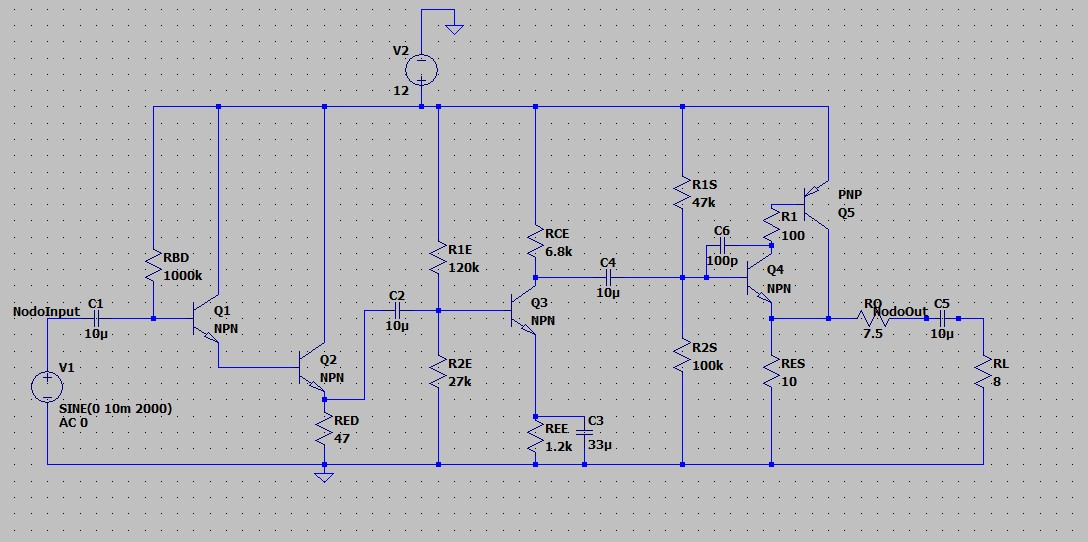
\includegraphics[width=0.85\linewidth]{Simu/Modelo_spice.jpg}
    \caption{Esquemático completo del amplificador en LTspice.}
    \label{fig:circuito_global}
\end{figure}

\vspace{0.5em}
{\small\textbf{Polarización y Disipación de Potencia Global (.op)}}

%\subsubsection{1.1. Polarización y Disipación de Potencia Global (.op)}
Se ejecuta la simulación \texttt{.op} para registrar los niveles de tensión en todos los nodos de la red y la corriente consumida desde la fuente principal $V_2 = 12\,\text{V}$ (\cref{PuntoOP}).
\begin{figure}[H]
    \centering
    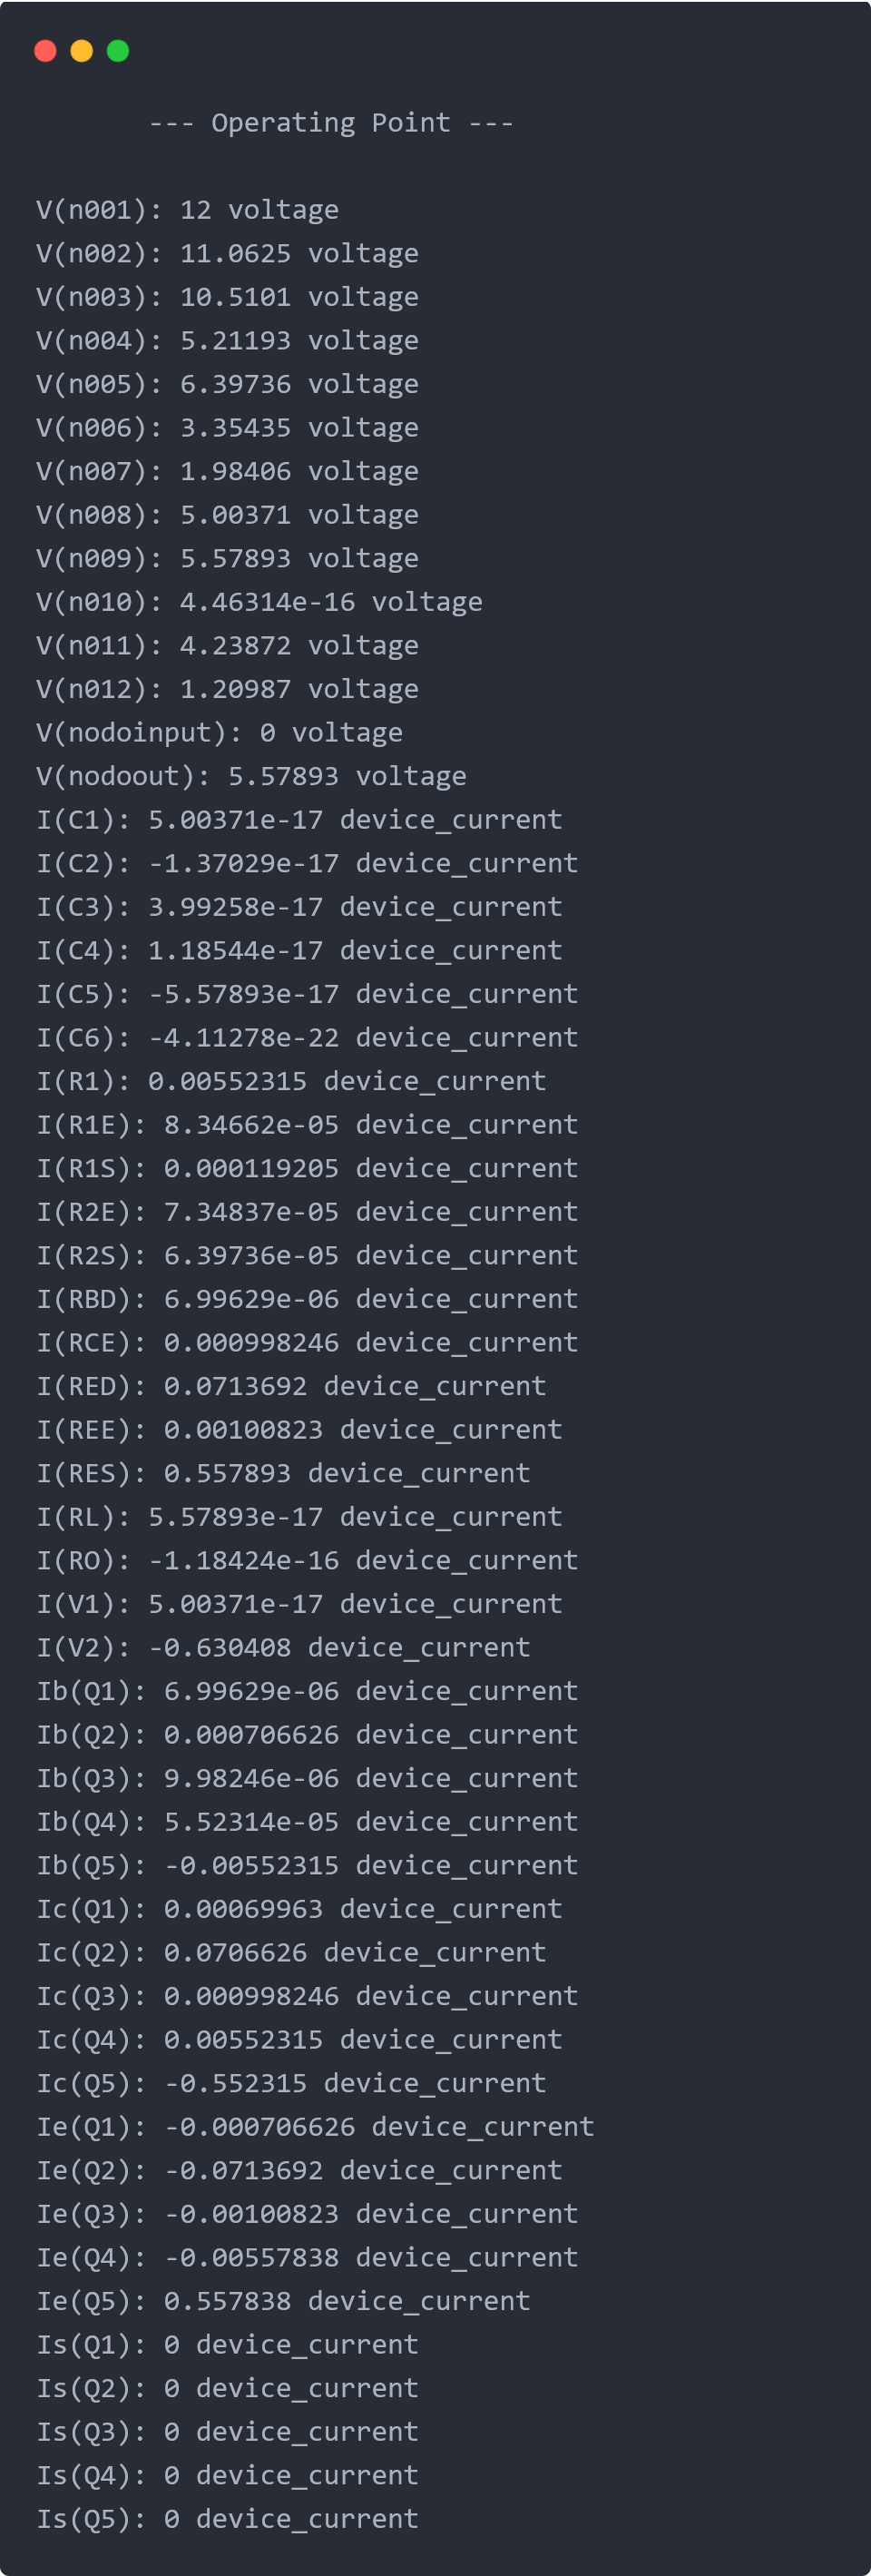
\includegraphics[width=0.5\linewidth]{Simu/OpTotal.png}
    \caption{Punto de operación.}
  \label{PuntoOP}
\end{figure}

\vspace{0.5em}
{\small\textbf{Impedancia de Entrada Total ($Z_{in}$)}}

%\subsubsection{1.2. Impedancia de Entrada Total ($Z_{in}$)}
Se mide aplicando un análisis \texttt{.ac} y calculando la relación entre la tensión en el nodo de entrada y la corriente entregada por la fuente $V_1$: $Z_{in} = \frac{V(\text{NodoInput})}{I(V1)}$ (\cref{SimuZin}).
\begin{figure}[H]
    \centering
    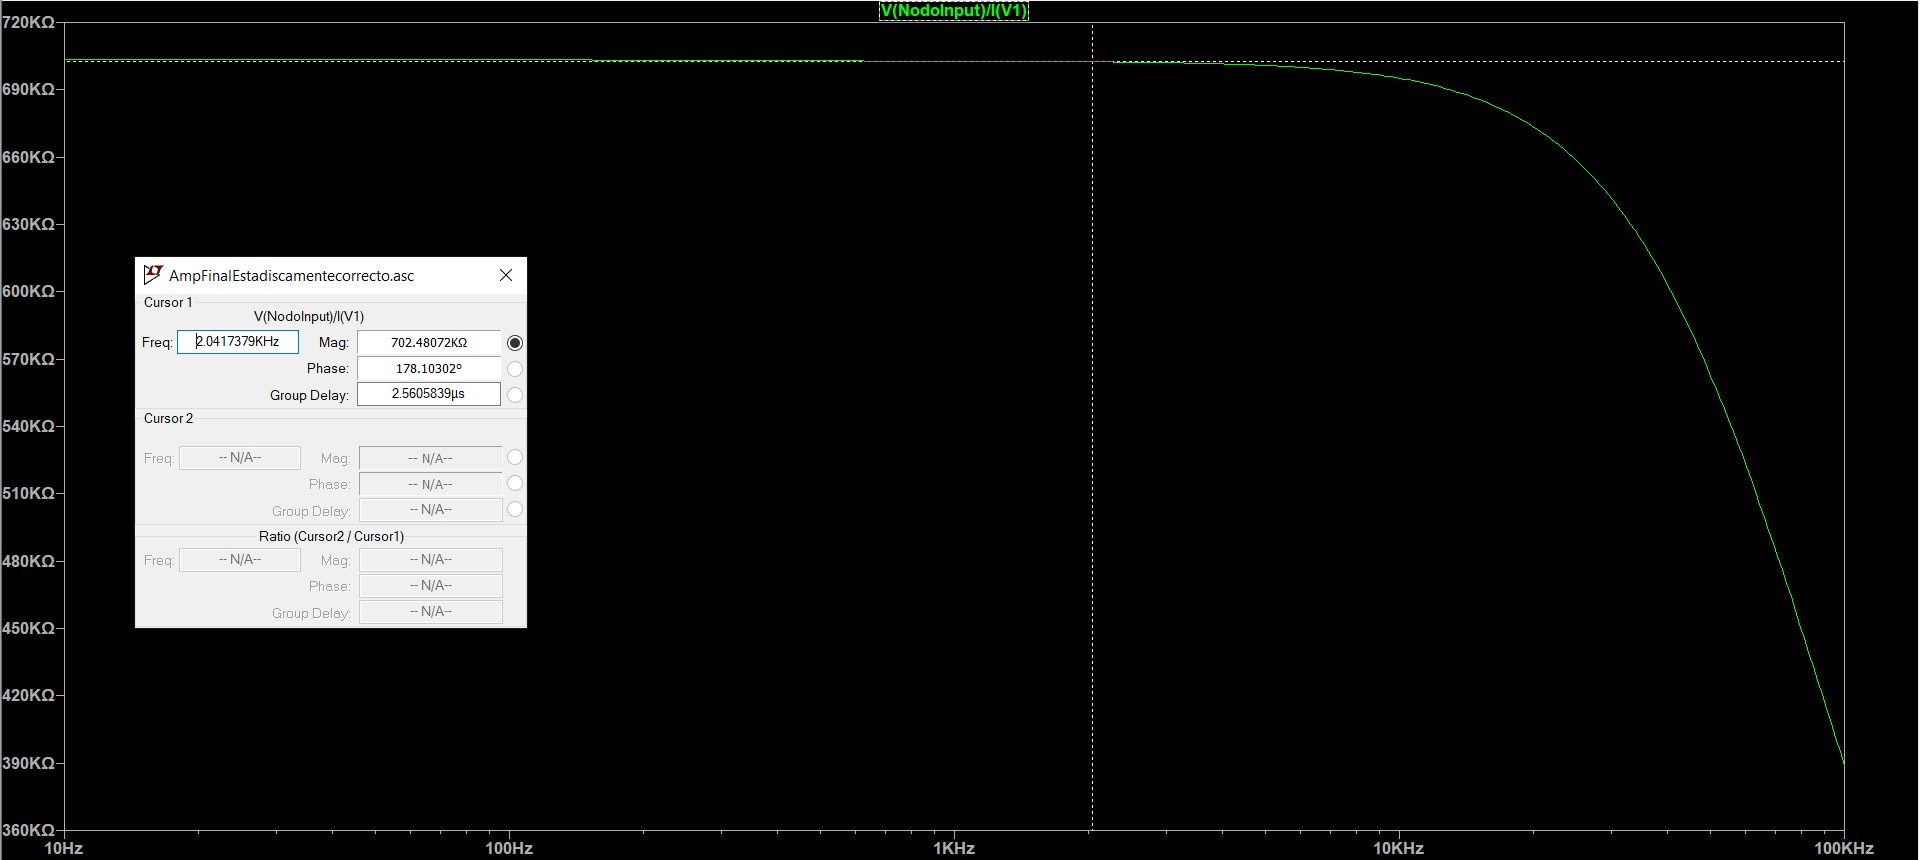
\includegraphics[width=0.75\linewidth]{Simu/Impedancia_Entrada_Total.jpg}
    \caption{Curva de la impedancia de entrada total del amplificador respecto a la frecuencia.}
  \label{SimuZin}
\end{figure}

\vspace{0.5em}
{\small\textbf{Impedancia de Salida Total ($Z_{out}$)}}

%\subsubsection{1.3. Impedancia de Salida Total ($Z_{out}$)}
Para medir la impedancia de salida global, se pasiva la fuente de entrada $V_1$ ($0\,\text{V}$ AC) y se aplica una fuente de corriente AC de prueba $I_{out} = 1\,\text{A}$ en el nodo de salida $\text{NodoOut}$, evaluando $Z_{out} = V(\text{NodoOut})$ (\cref{SimuZo}, \cref{SimuZoT}).
\begin{figure}[H]
    \centering
    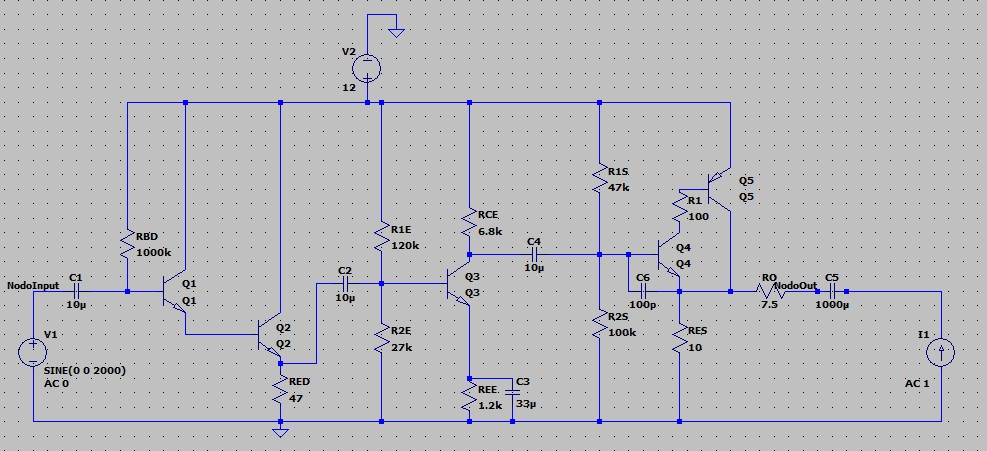
\includegraphics[width=0.75\linewidth]{Simu/Impedancia_Salida_Ciurcuito.jpg}
    \caption{Circuito de como fue medida la impedancia de salida.}
    \label{SimuZo}
\end{figure}
\begin{figure}[H]
    \centering
    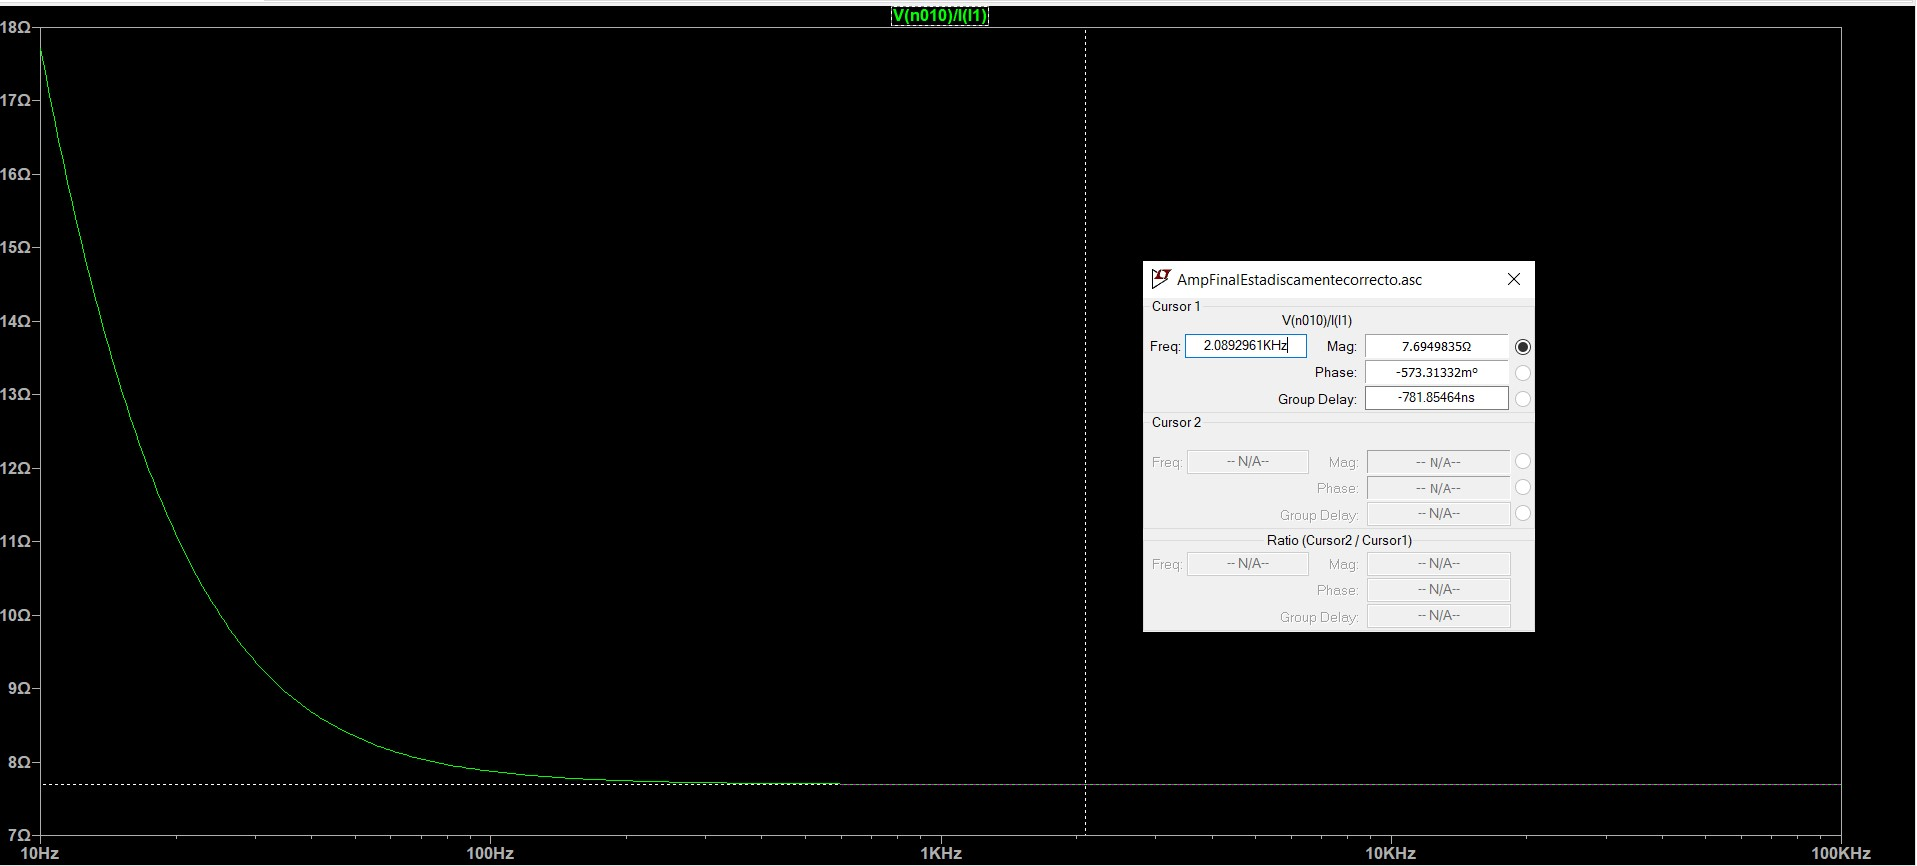
\includegraphics[width=0.75\linewidth]{Simu/Impedancia_Salida_tetal.jpg}
    \caption{Montaje y simulación de la impedancia de salida global $Z_{out}$ del circuito.}
  \label{SimuZoT}
\end{figure}

\vspace{0.5em}
{\small\textbf{Respuesta en Frecuencia AC ($A_v$)}}

%\subsubsection{1.4. Respuesta en Frecuencia AC ($A_v$)}
Análisis del ancho de banda y ganancia total de tensión midiendo $A_v = \frac{V(\text{NodoOut})}{V(\text{NodoInput})}$ (\cref{LimDer}, \cref{LimIz}).
\begin{figure}[H]
    \centering
    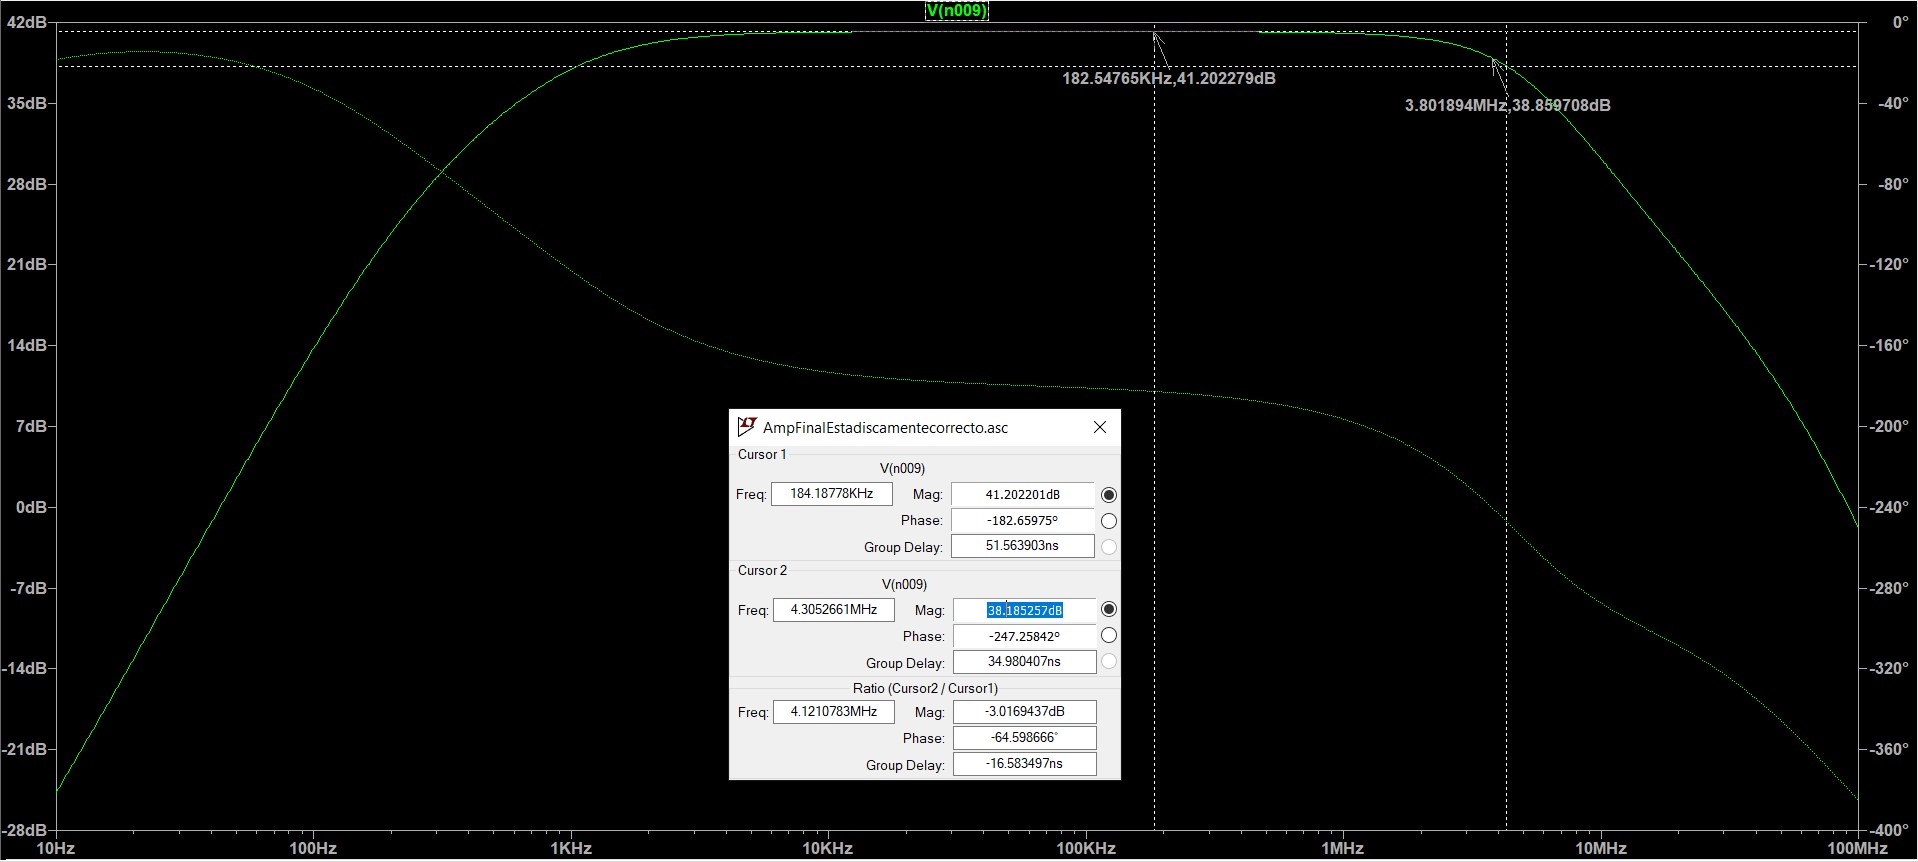
\includegraphics[width=0.75\linewidth]{Simu/BW-LimiteDerecho.jpg}
    \caption{Respuesta en frecuencia con cursor en limite derecho.}
    \label{LimDer}
\end{figure}
\begin{figure}[H]
    \centering
    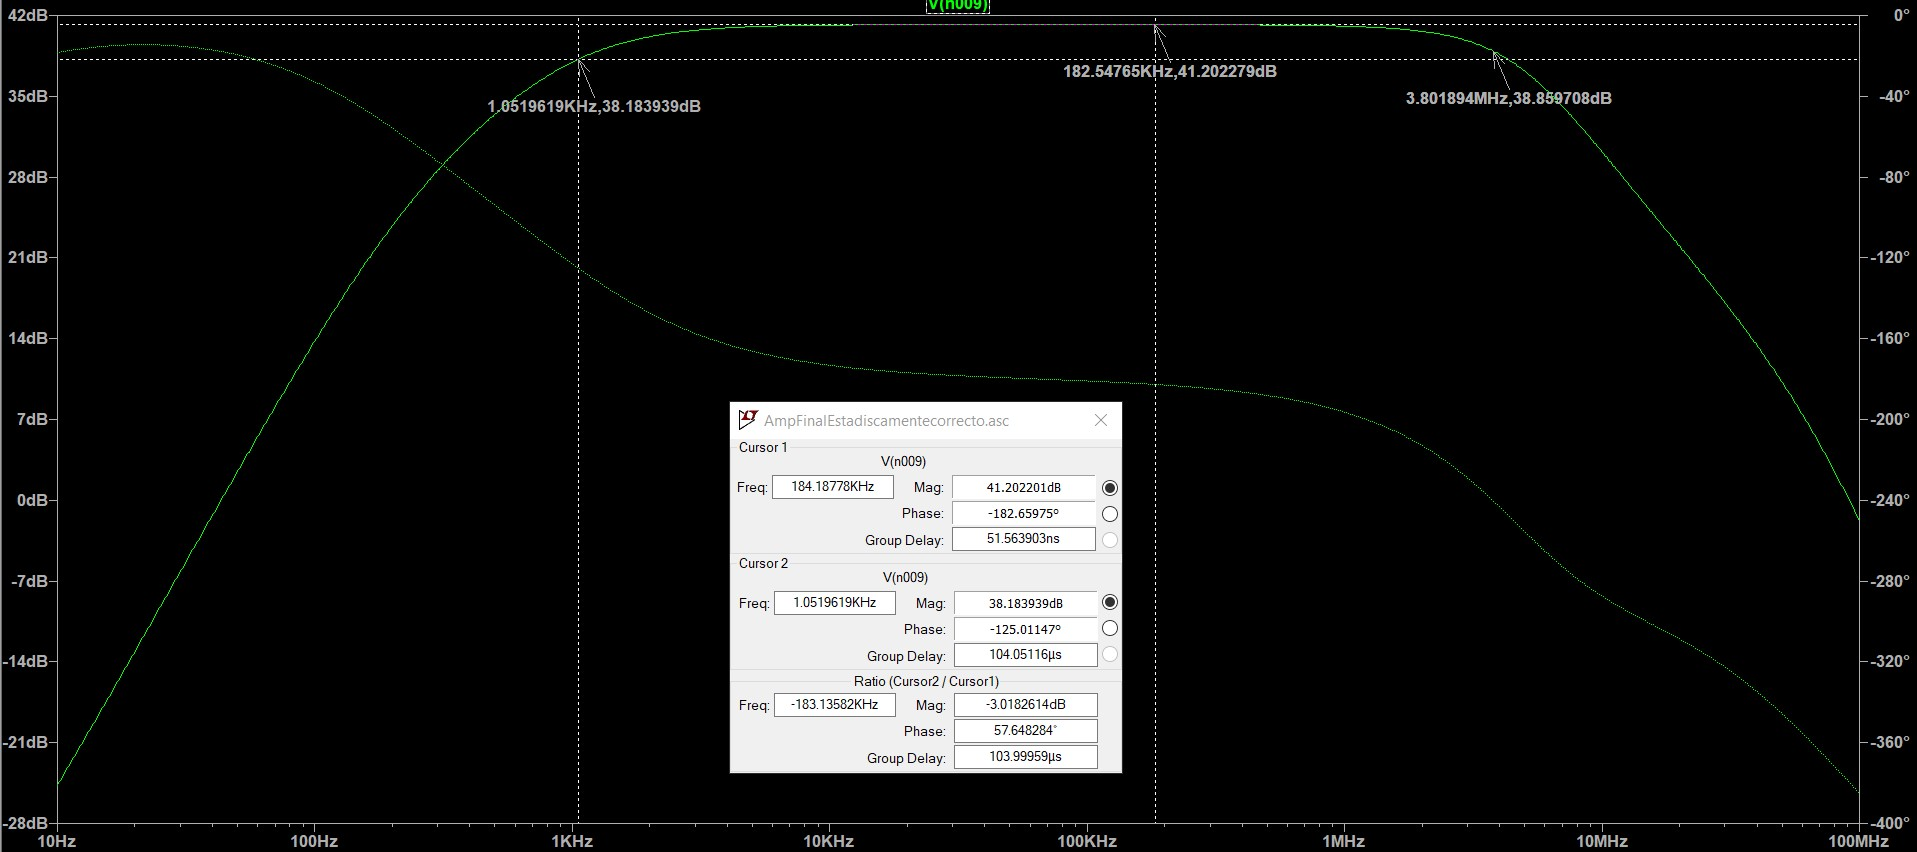
\includegraphics[width=0.75\linewidth]{Simu/BW-LimiteIzquierdo.jpg}
    \caption{Respuesta en frecuencia con cursor en limite izquierdo.}
  \label{LimIz}
\end{figure}

\vspace{0.5em}
{\small\textbf{Respuesta Temporal (.tran)}}

%\subsubsection{1.5. Respuesta Temporal (.tran)}
Respuesta en el dominio del tiempo frente a una entrada senoidal de $5\,\text{kHz}$ e intensidad $10\,\text{mV}_{\text{pico}}$. Se evalúa la excursión de tensión y la simetría de la onda sobre el nodo de salida (\cref{SimuVo}).
\begin{figure}[H]
    \centering
    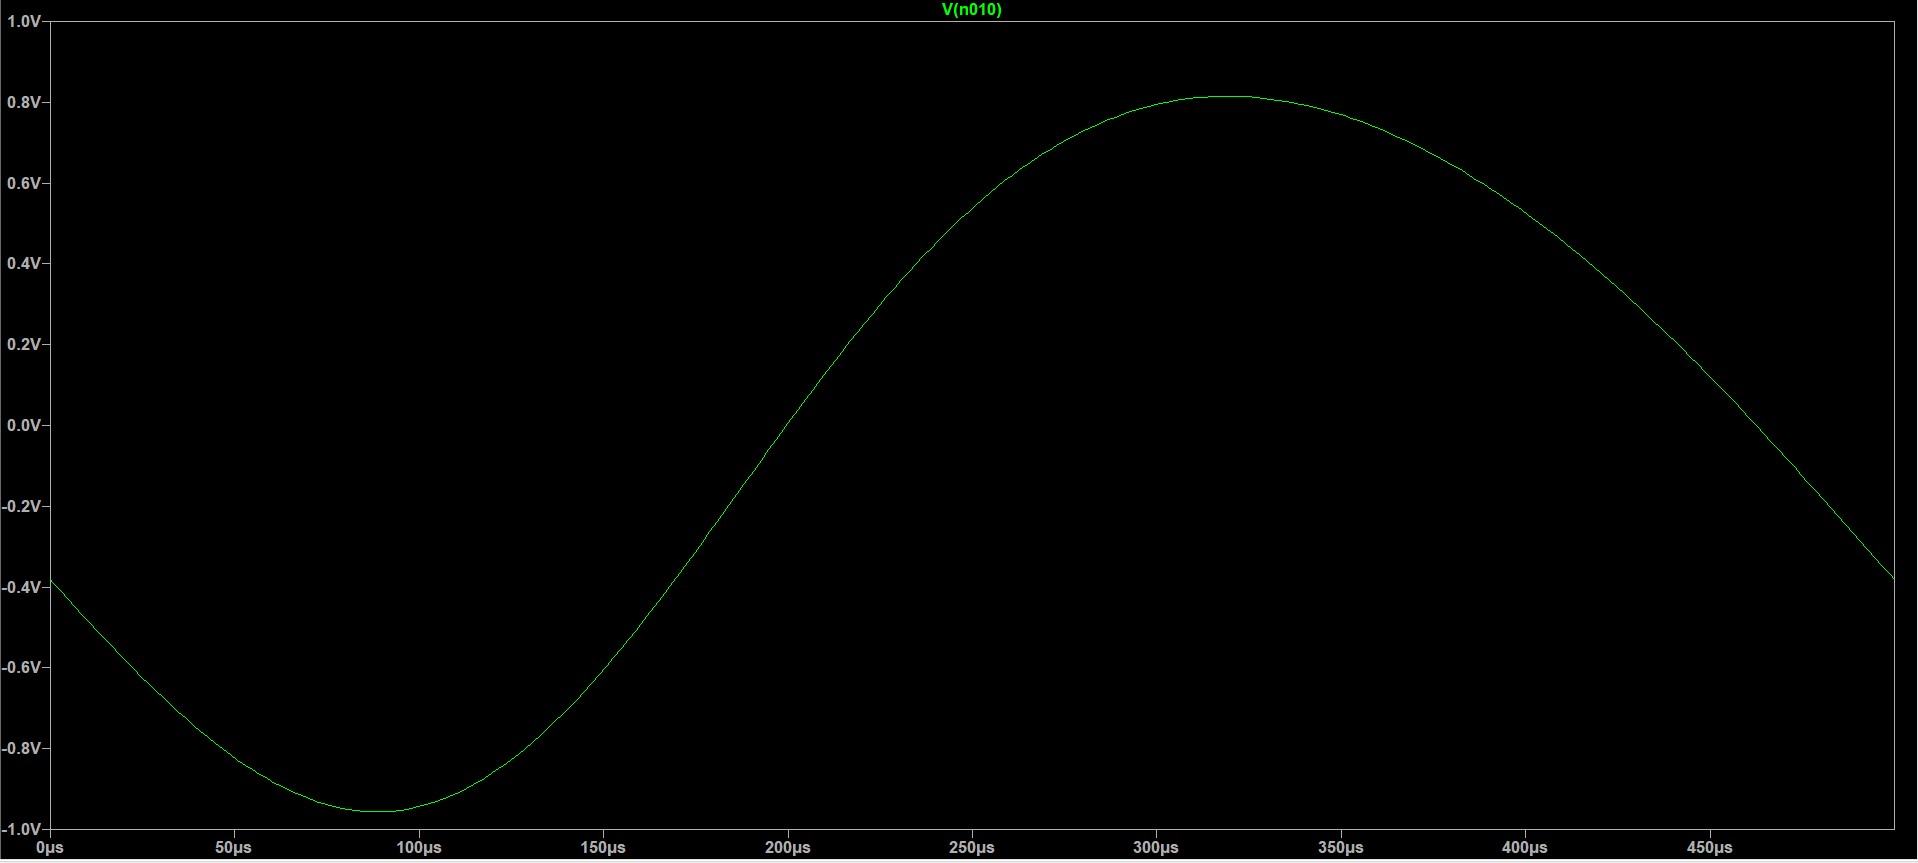
\includegraphics[width=0.75\linewidth]{Simu/Voltaje_salida_10m.jpg}
    \caption{Medición de la respuesta temporal (.tran) de la tensión de salida sobre la carga de $8\,\Omega$.}
  \label{SimuVo}
\end{figure}

\vspace{0.5em}
{\small\textbf{Densidad Espectral de Potencia del Ruido (PSD .noise)}}

%\subsubsection{1.6. Densidad Espectral de Potencia del Ruido (PSD .noise)}
Medición de la PSD de ruido referida a la salida del sistema completo mediante \texttt{.noise V(NodoOut) V1 dec 100 10 100k} (\cref{SimuPSD}, \cref{SimuPSDT}).
\begin{figure}[H]
    \centering
    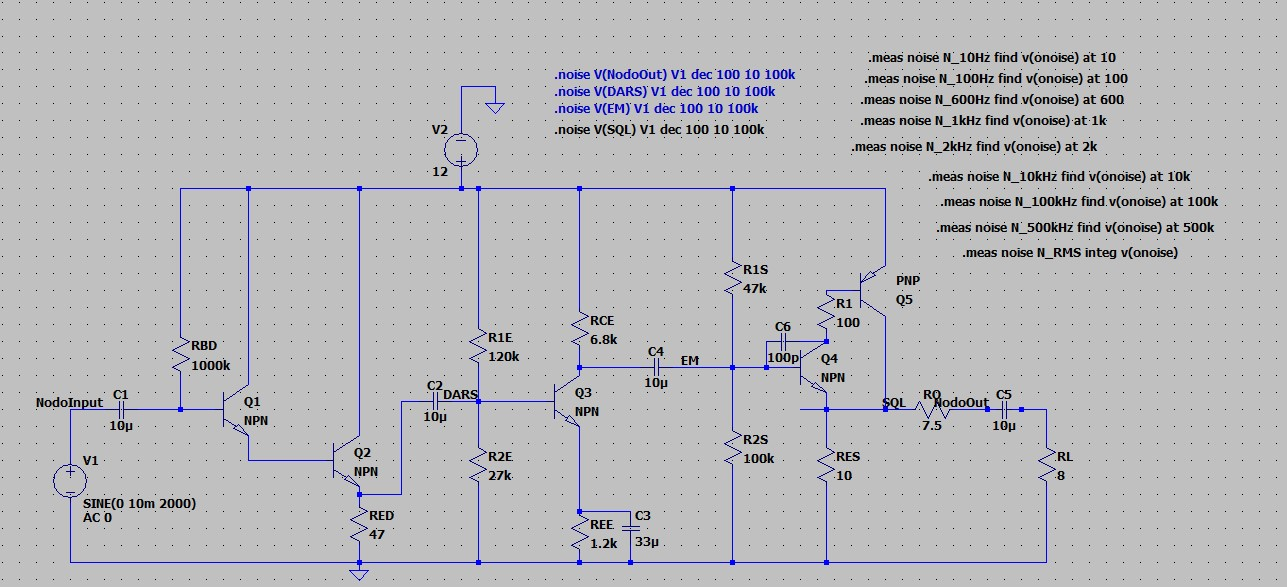
\includegraphics[width=0.75\linewidth]{Simu/Noise-totalcondirct.jpg}
    \caption{Circuito representativo de como se midió el PSD.}
  \label{SimuPSD}
\end{figure}\begin{figure}[H]
    \centering
    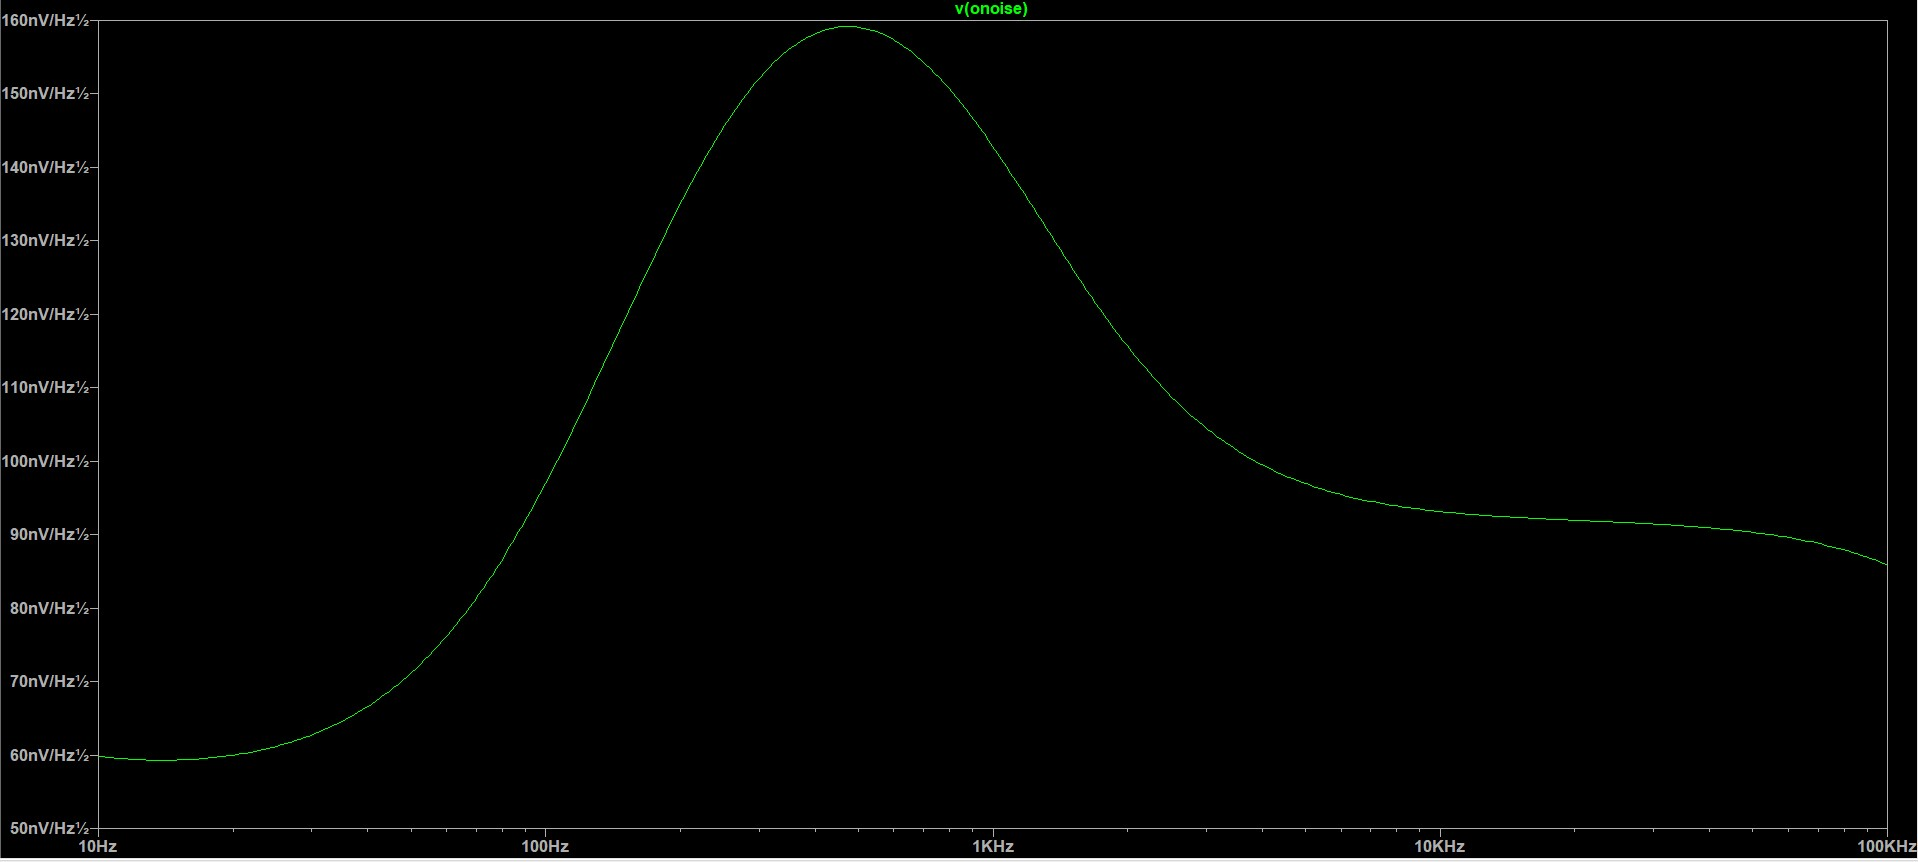
\includegraphics[width=0.75\linewidth]{Simu/Noise-out.jpg}
    \caption{Densidad espectral de potencia del ruido (PSD) total a la salida.}
  \label{SimuPSDT}
\end{figure}

\vspace{0.5em}
{\small\textbf{Distorsión Armónica Total (THD via FFT / .four)}}

%\subsubsection{1.7. Distorsión Armónica Total (THD via FFT / .four)}
Se aplica el análisis de Fourier mediante la directiva \texttt{.four 2000 V(NodoOut)} sobre la señal en la carga $R_L$ a $2\,\text{kHz}$. Los resultados numéricos de distorsión armónica total y la amplitud de las componentes armónicas individuales se inspeccionaron directamente en el registro de salida de LTspice (\textit{Spice Error Log}), al cual se accede mediante la combinación de teclas \textbf{\texttt{Ctrl + L}} tras completar la simulación de transitorios (\cref{THD}).

\begin{figure}[H]
    \centering
    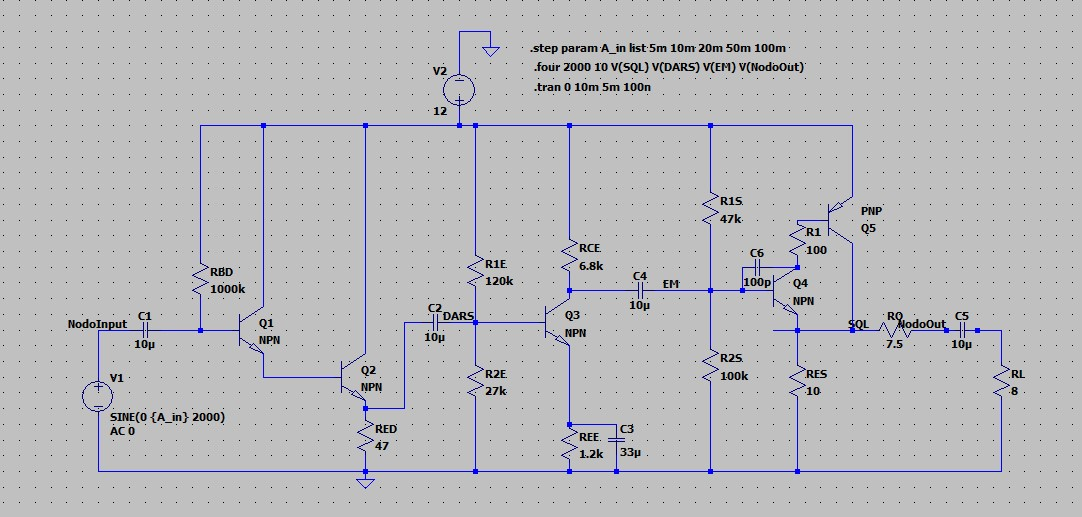
\includegraphics[width=0.75\linewidth]{Simu/Med-THD.jpg}
    \caption{Esquemático y configuración del análisis de Fourier (.four) en LTspice para la inspección de resultados de THD vía Error Log}
  \label{THD}
\end{figure}

\vspace{0.5em}
{\small\textbf{Evaluación de Límites de Operación y Pérdida de Linealidad}}

%\subsubsection{1.8. Evaluación de Límites de Operación y Pérdida de Linealidad}
Para caracterizar con precisión los márgenes dinámicos del amplificador completo y determinar el punto exacto donde se pierde la linealidad (recorte por saturación o corte), se implementaron barridos paramétricos utilizando la directiva \texttt{.step}. Los resultados se estructuran en los siguientes tres análisis:

{\small\textbf{1- Pérdida de Linealidad por Variación de Amplitud de Entrada ($V_{in}$)}}

Mediante el comando \texttt{.step param A\_in list 5m 10m 15m 17m 20m}, se incrementó progresivamente la amplitud de la señal de entrada, observando en la señal de salida el instante exacto en que la forma de onda deja de ser puramente senoidal y comienza el recorte (\cref{PerLinME}. \cref{TransfDin}).

\begin{figure}[H]
    \centering
    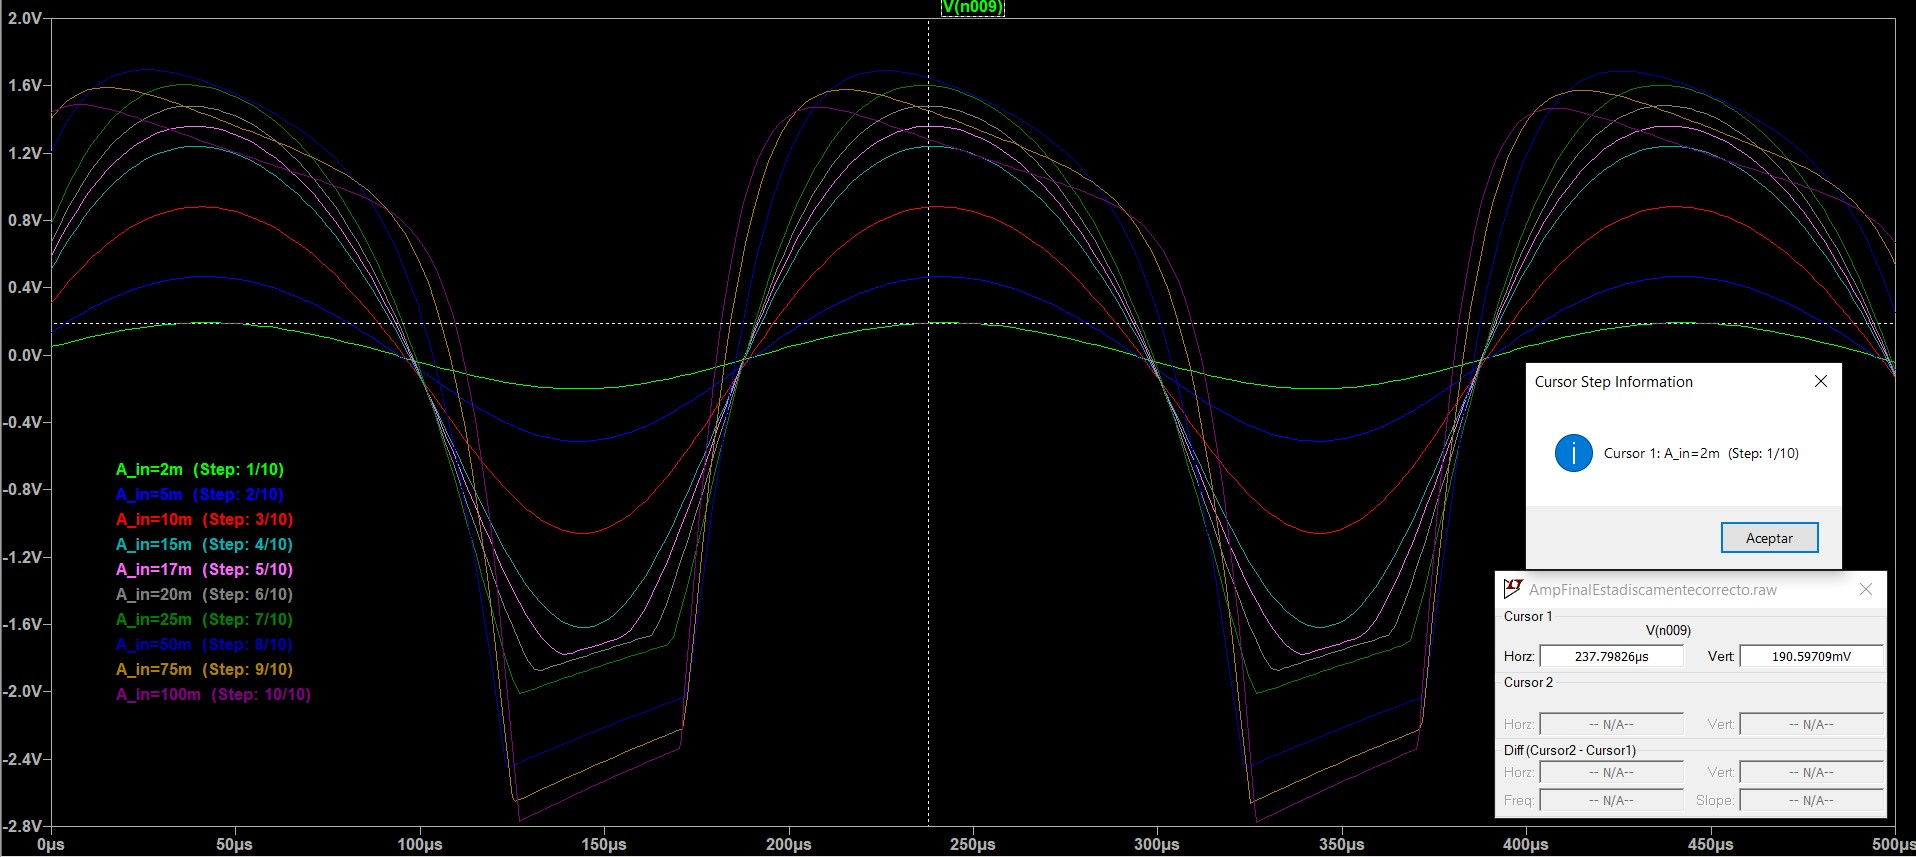
\includegraphics[width=0.75\linewidth]{Simu/Voltaje_salida_5k.jpg}
    \caption{Evaluación de la pérdida de linealidad por excursión máxima de la señal de entrada $V_{in}$.}
  \label{PerLinME}
\end{figure}
\begin{figure}[H]
    \centering
    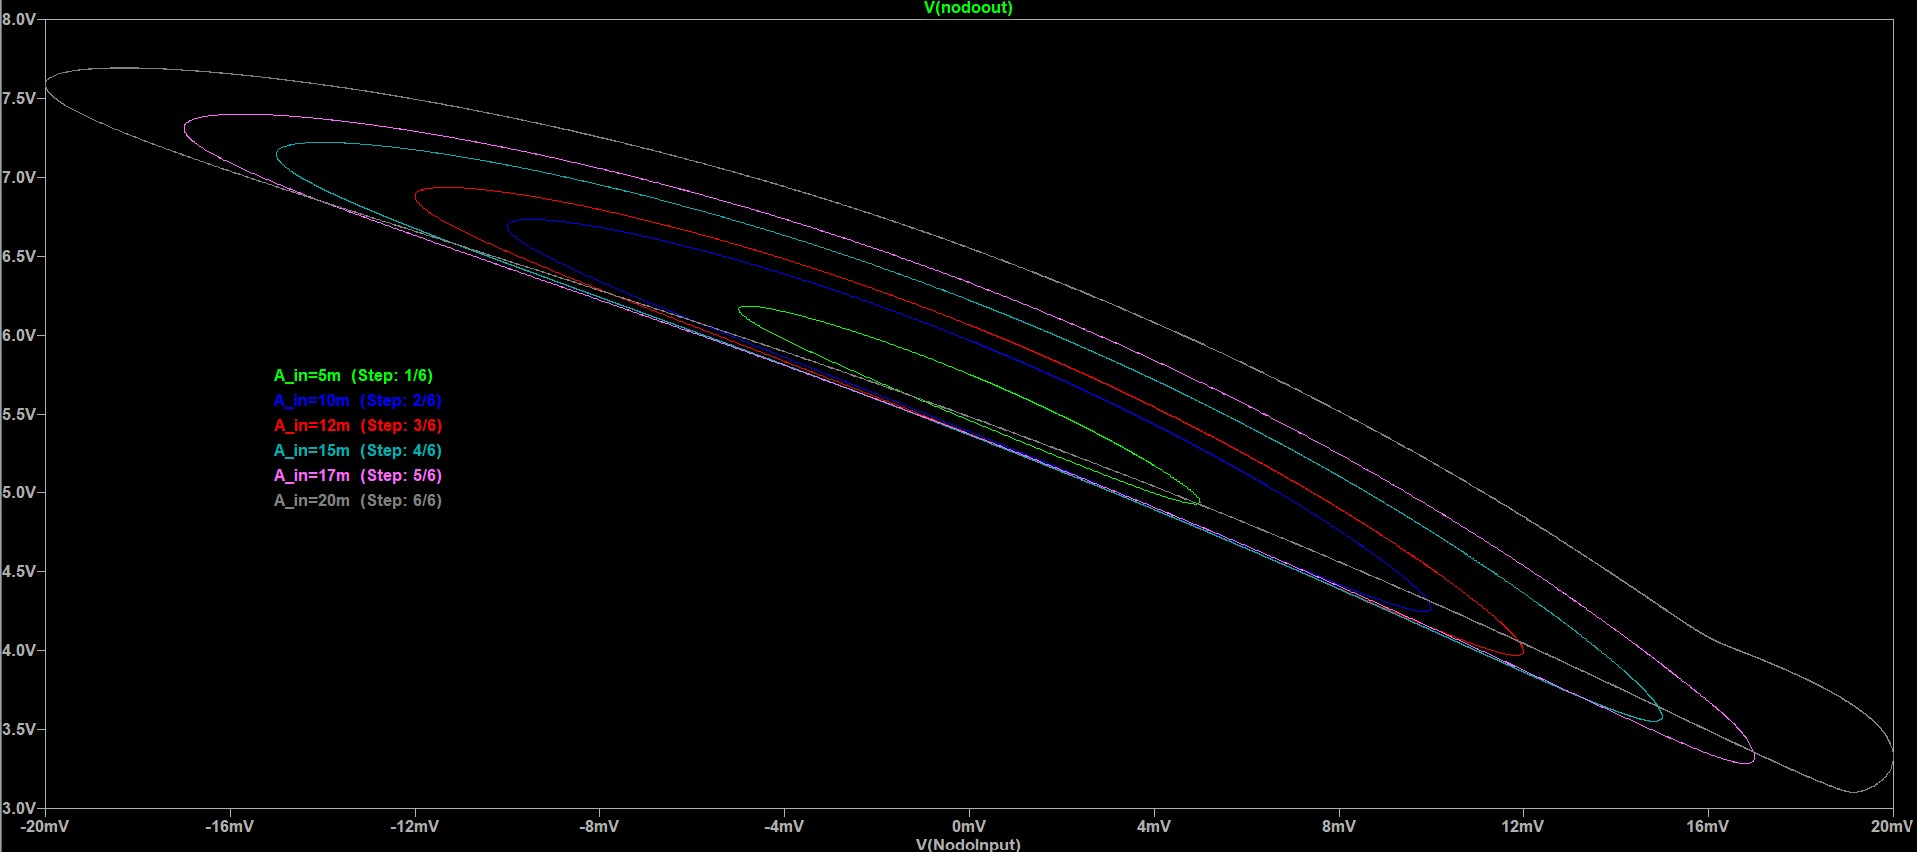
\includegraphics[width=0.75\linewidth]{Simu/Linealidad.jpg}
    \caption{Curva de transferencia dinámica $V(\text{NodoOut})$ vs. $V(\text{NodoInput})$ para diferentes amplitudes de entrada ($A_{in}$ de $5\,\text{mV}$ a $20\,\text{mV}$). La pendiente e inclinación representan la ganancia invertida del sistema, mientras que la deformación progresiva en los bordes para $A_{in} \ge 17\,\text{mV}$ evidencia la pérdida de linealidad y la presencia de distorsión armónica.}
    \label{TransfDin}
\end{figure}

{\small\textbf{2- Límites de Operación por Variación de Alimentación ($V_{CC}$ hacia arriba y hacia abajo)}}

%\paragraph{1.8.2. Límites de Operación por Variación de Alimentación ($V_{CC}$ hacia arriba y hacia abajo)}
Se analizó la tolerancia del amplificador variando la fuente de alimentación $V_2$ ($V_{CC}$) mediante \texttt{.step param VCC 6 18 1}. Esto permitió determinar la tensión mínima de alimentación ($V_{CC,min}$) necesaria para mantener los transistores en región activa y la tensión máxima ($V_{CC,max}$) antes de superar los límites de disipación o distorsión (\cref{BarridoAbajo}, \cref{BarridoArriba}).

\begin{figure}[H]
    \centering
    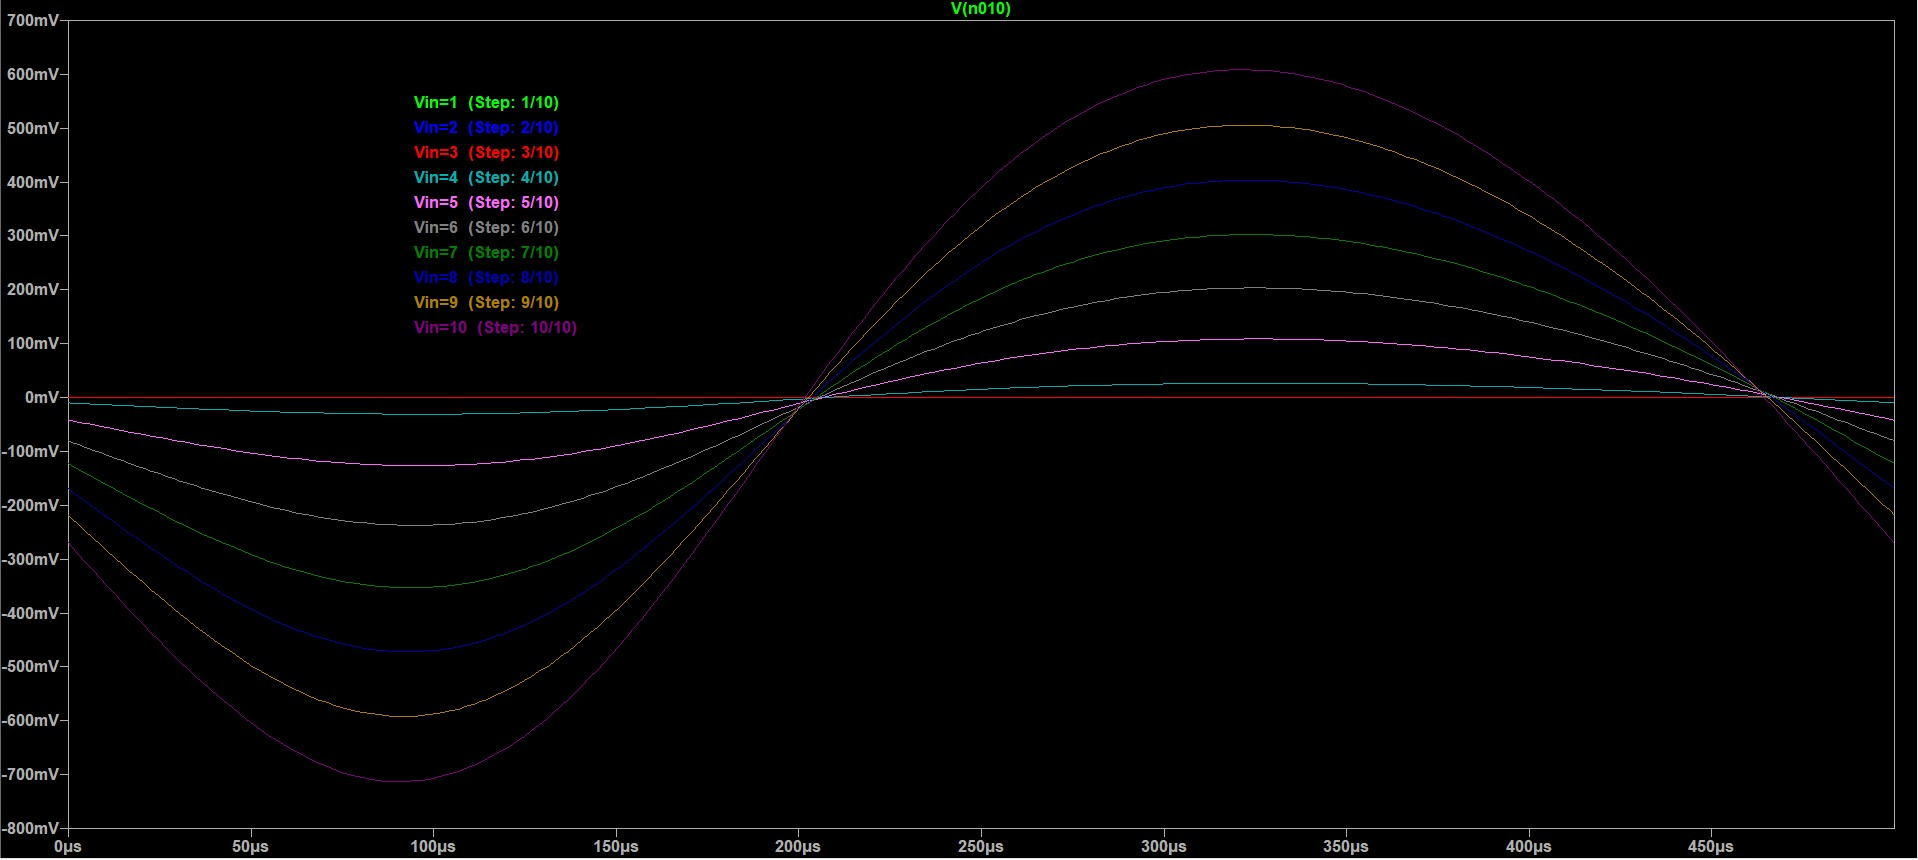
\includegraphics[width=0.75\linewidth]{Simu/voltajemuerteabajototal-salida.jpg}
    \caption{Comportamiento de la señal de salida ante la variación de la fuente de alimentación $V_{CC}$ (barrido hacia abajo).}
  \label{BarridoAbajo}
\end{figure}
\begin{figure}[H]
    \centering
    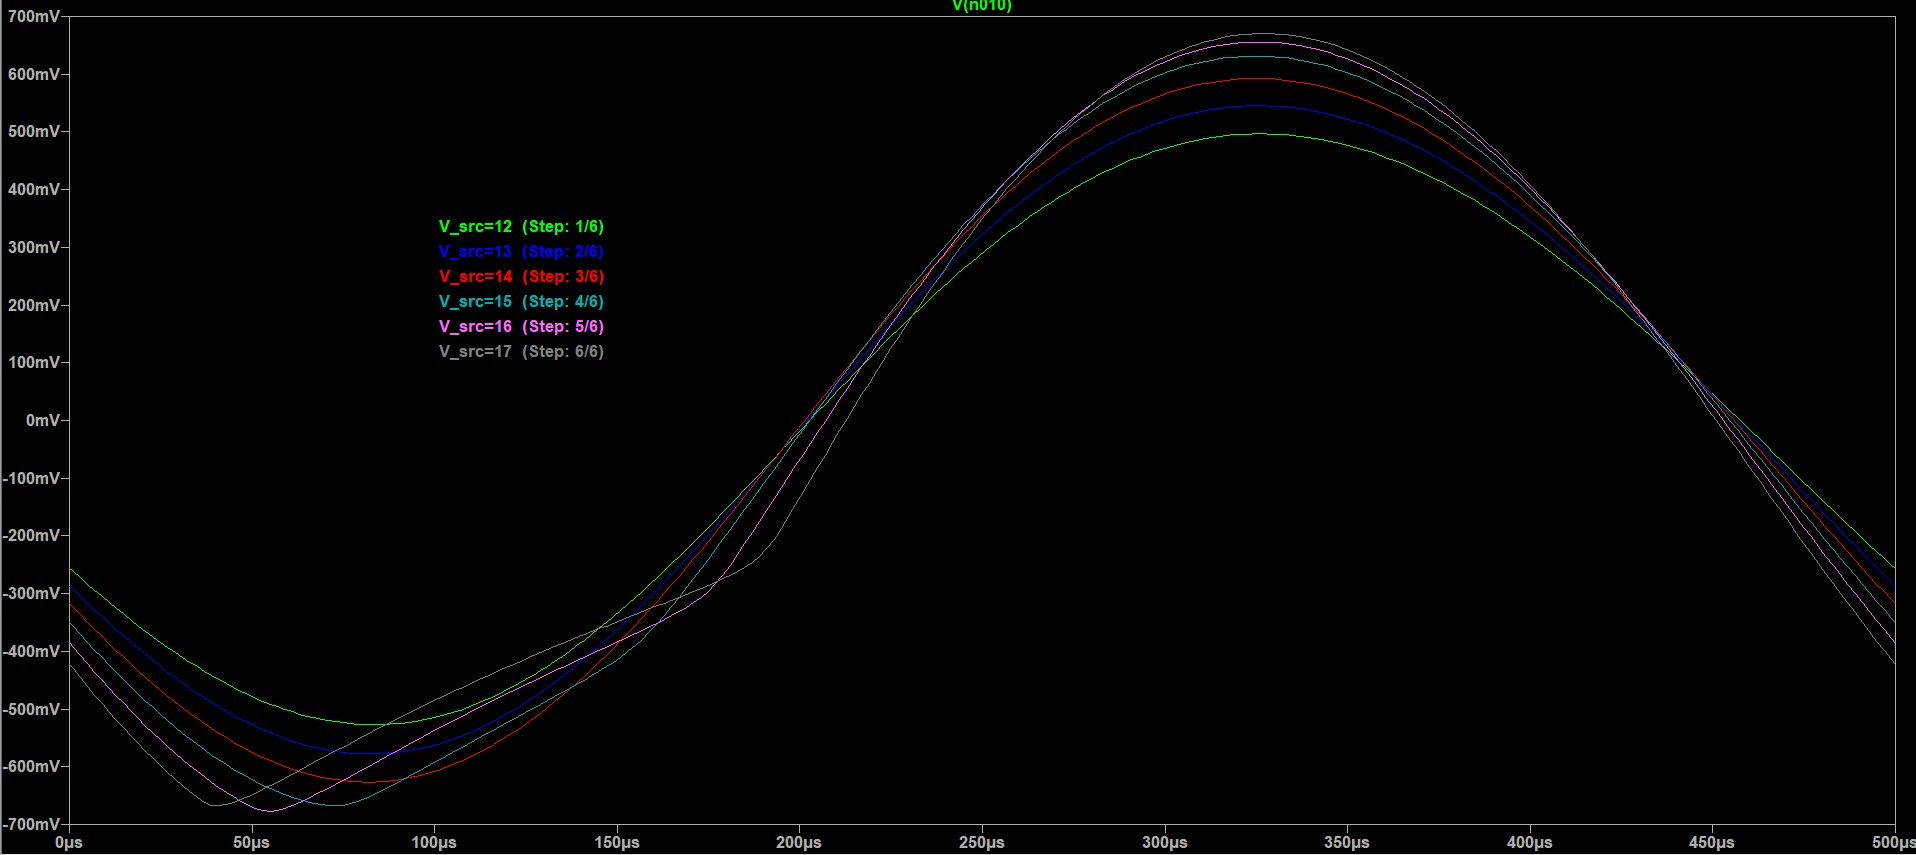
\includegraphics[width=0.75\linewidth]{Simu/voltajemuertearribatotal-salida.jpg}
    \caption{Comportamiento de la señal de salida ante la variación de la fuente de alimentación $V_{CC}$ (barrido hacia arriba).}
  \label{BarridoArriba}
\end{figure}

{\small\textbf{3- Límites de Operación por Variación de Carga ($R_L$)}}

%\paragraph{1.8.3. Límites de Operación por Variación de Carga ($R_L$)}
Se realizó un barrido sobre la impedancia de salida utilizando \texttt{.step param RL 4 16 2} para evaluar la capacidad de entrega de corriente del amplificador y determinar el rango de impedancias de carga sobre el cual se preserva la respuesta lineal sin recorte por corriente (\cref{GainRo}).

\begin{figure}[H]
    \centering
    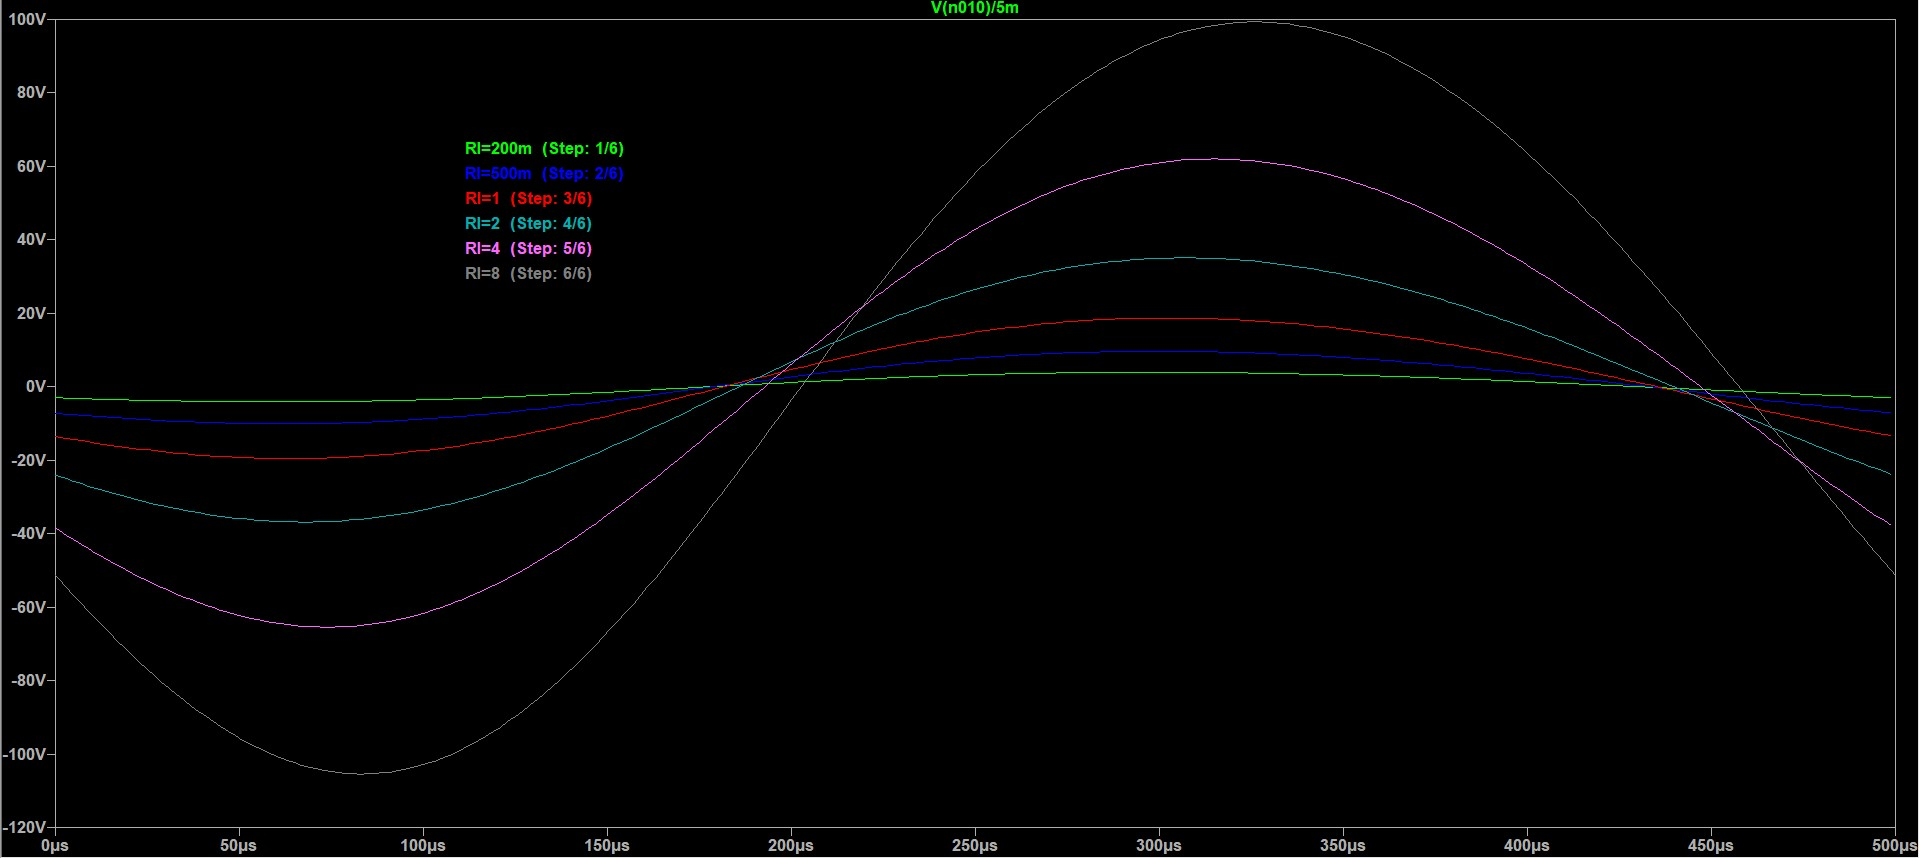
\includegraphics[width=0.75\linewidth]{Simu/RLMURTESALIDA.jpg}
    \caption{Ganancia frente a variaciones en la resistencia de carga $R_L$.}
  \label{GainRo}
\end{figure}

% =========================================================================
% APARTADO 2: ETAPA DARLINGTON
% =========================================================================
\subsubsection{Primera Etapa: Adaptador de Entrada Darlington ($Q_1$ - $Q_2$)}
%\section{2. Primera Etapa: Adaptador de Entrada Darlington ($Q_1$ - $Q_2$)}

\begin{figure}[H]
    \centering
    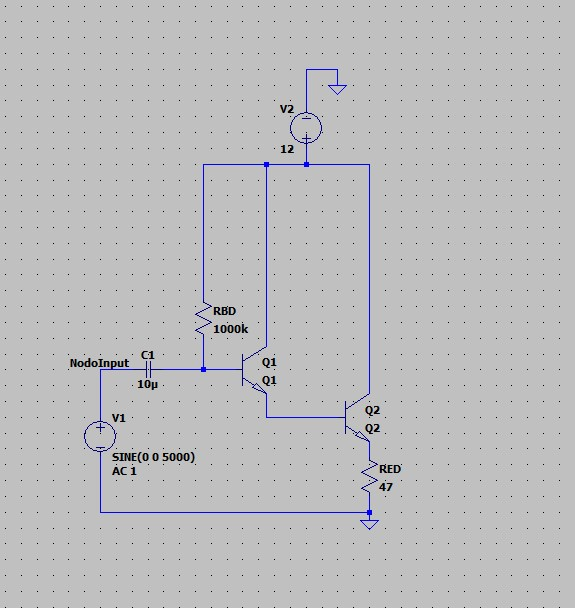
\includegraphics[width=0.45\linewidth]{Simu/Darlinton.jpg}
    \caption{Circuito esquemático de la etapa Darlington aislada.}
\end{figure}

\vspace{0.5em}
{\small\textbf{Polarización y Disipación de Potencia}}

%\subsubsection{2.1. Polarización y Disipación de Potencia}
Se determinó el punto estático mediante \texttt{.op}, evaluando las corrientes de colector y las tensiones $V_{CE}$ para calcular la disipación estática de $Q_1$ y $Q_2$.
\begin{verbatim}
.op
.meas DC VCE_Q1 PARAM V(vcc)-V(e1)
.meas DC IC_Q1 I(Q1)
.meas DC P_Q1 PARAM VCE_Q1*IC_Q1
\end{verbatim}

\vspace{0.5em}
{\small\textbf{Medición de Impedancias de la Etapa Darlington ($Z_{in1}$ y $Z_{out1}$)}}

%\subsubsection{2.2. Medición de Impedancias de la Etapa Darlington ($Z_{in1}$ y $Z_{out1}$)}
La impedancia de entrada $Z_{in1}$ se midió inyectando señal desde la fuente de entrada $V_1$. Para la impedancia de salida $Z_{out1}$, se aisló la etapa, se pasivó la entrada y se colocó una fuente de prueba $I_{test}$ en el emisor de $Q_2$.

\paragraph{Impedancia de Entrada ($Z_{in1}$)} 
Se puede ver en (\cref{SimuZin1}).
\begin{figure}[H]
    \centering
    \begin{minipage}{0.48\textwidth}
        \centering
        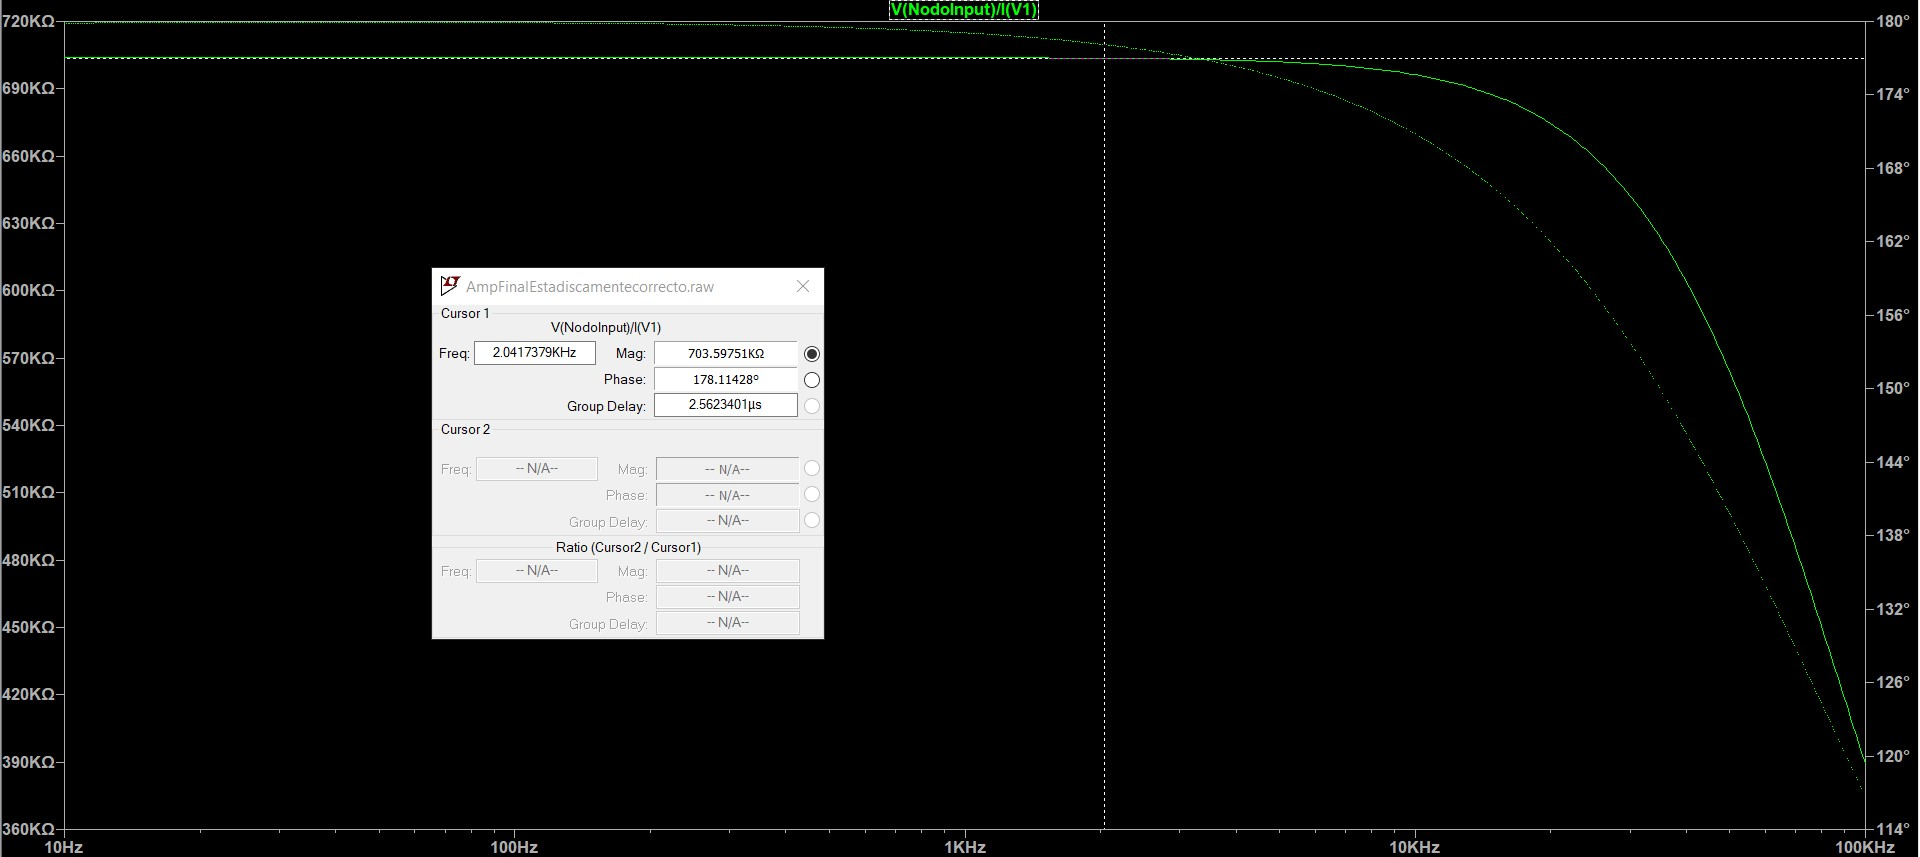
\includegraphics[width=\linewidth]{Simu/ImpedanciaIN_Darlinton.jpg}
        \caption{Curva de respuesta $Z_{in1}$.}
    \label{SimuZin1}
    \end{minipage}
\end{figure}

\paragraph{Impedancia de Salida ($Z_{out1}$)} 
Se puede ver en (\cref{SimuZout1}).
\begin{figure}[H]
    \centering
    \begin{minipage}{0.48\textwidth}
        \centering
        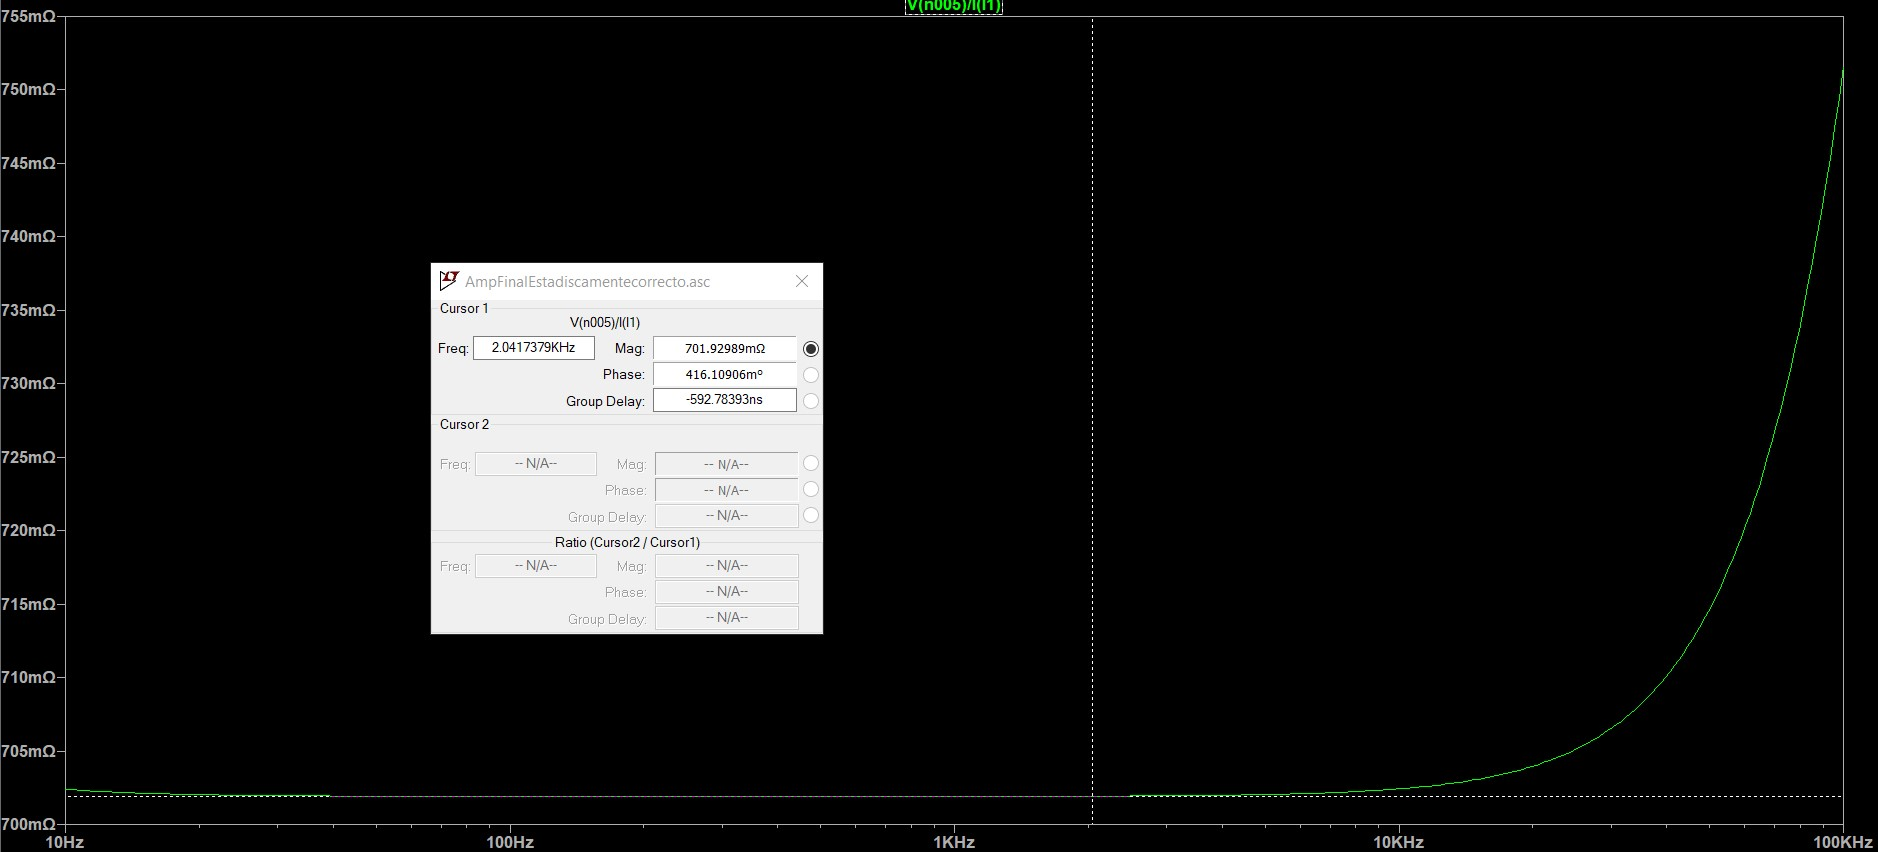
\includegraphics[width=\linewidth]{Simu/ImpedanciaOUT_Darlinton.jpg}
        \caption{Curva de respuesta de $Z_{out1}$.}
  \label{SimuZout1}
    \end{minipage}
\end{figure}

\vspace{0.5em}
{\small\textbf{Respuesta en Frecuencia, Temporal, Ruido y Linealidad}}

%\subsubsection{2.3. Respuesta en Frecuencia, Temporal, Ruido y Linealidad}
Se caracterizó la respuesta frecuencial mediante barrido \texttt{.ac}, la excursión temporal con \texttt{.tran}, la PSD de ruido a la salida de la etapa con \texttt{.noise} y la respuesta dinámica X-Y con \texttt{.step param A\_in} (\cref{SimuBW}, \cref{SimuVtemp}, \cref{SimuPSDDar}, \cref{SimuLinDar}).

\begin{figure}[H]
    \centering
    \begin{minipage}{0.48\textwidth}
        \centering
        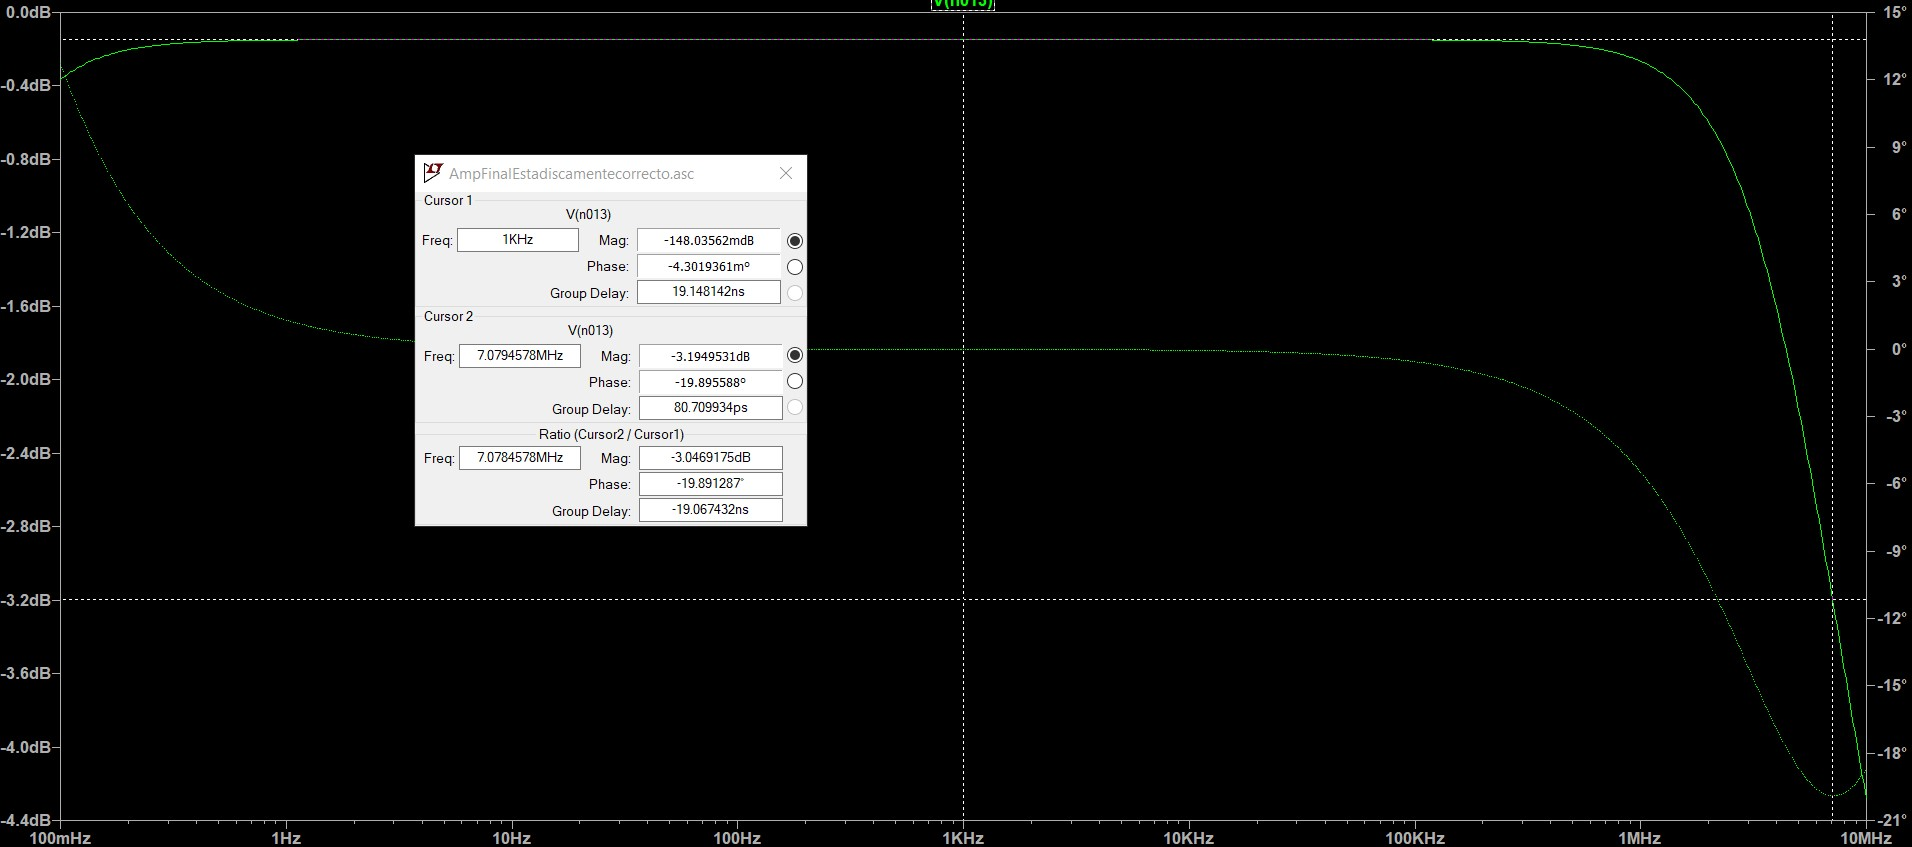
\includegraphics[width=\linewidth]{Simu/BW-DARLINTONG-DB.jpg}
        \caption{Respuesta AC (Ancho de banda).}
      \label{SimuBW}
    \end{minipage}\hfill
    \begin{minipage}{0.48\textwidth}
        \centering
        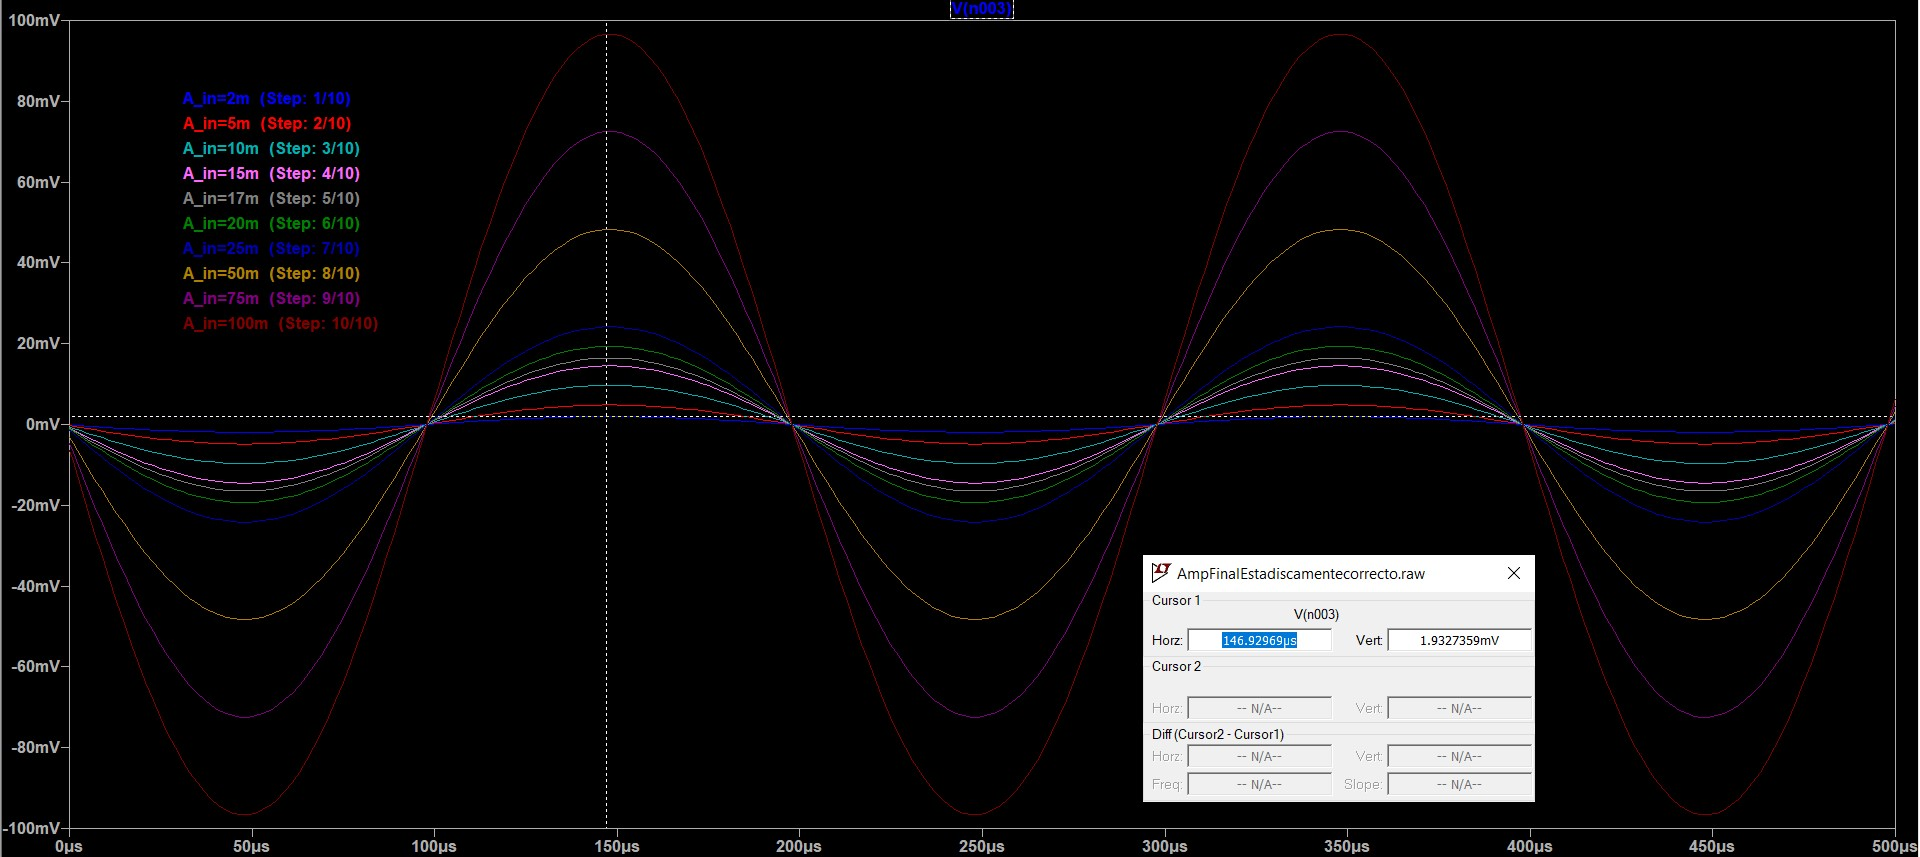
\includegraphics[width=\linewidth]{Simu/Voutppdarlin.jpg}
        \caption{Tensión temporal pico a pico.}
      \label{SimuVtemp}
    \end{minipage}
\end{figure}

\begin{figure}[H]
    \centering
    \begin{minipage}{0.48\textwidth}
        \centering
        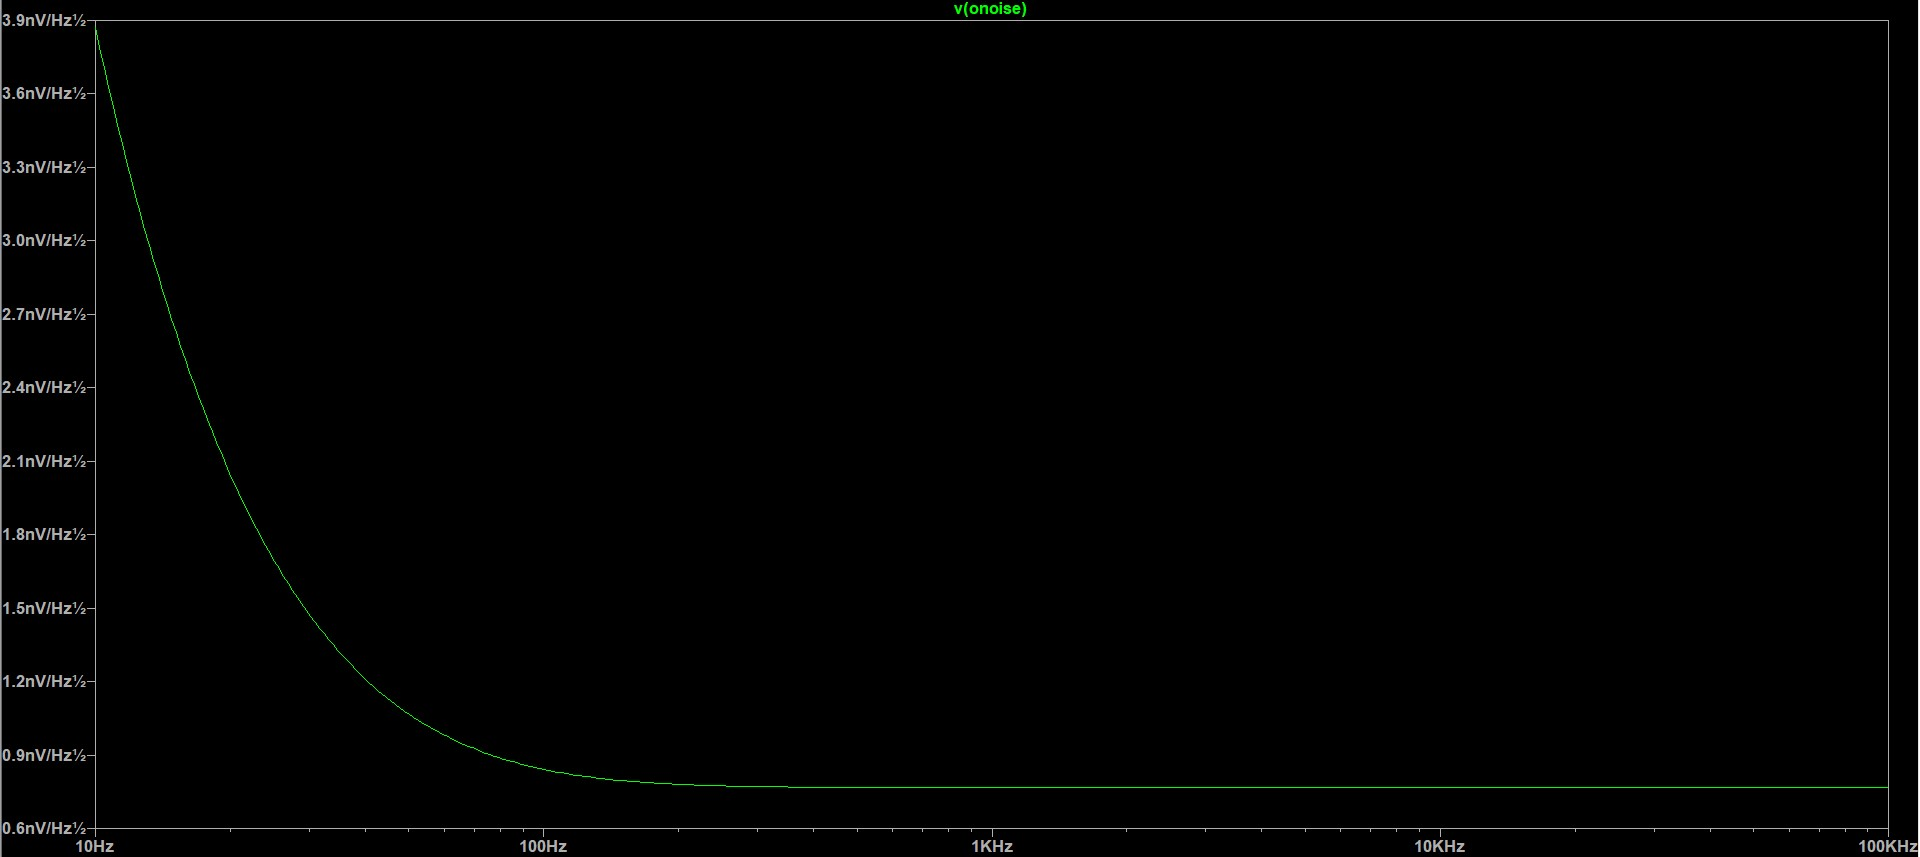
\includegraphics[width=\linewidth]{Simu/Noise-dar.jpg}
        \caption{PSD de Ruido - Darlington.}
      \label{SimuPSDDar}
    \end{minipage}\hfill
    \begin{minipage}{0.48\textwidth}
        \centering
        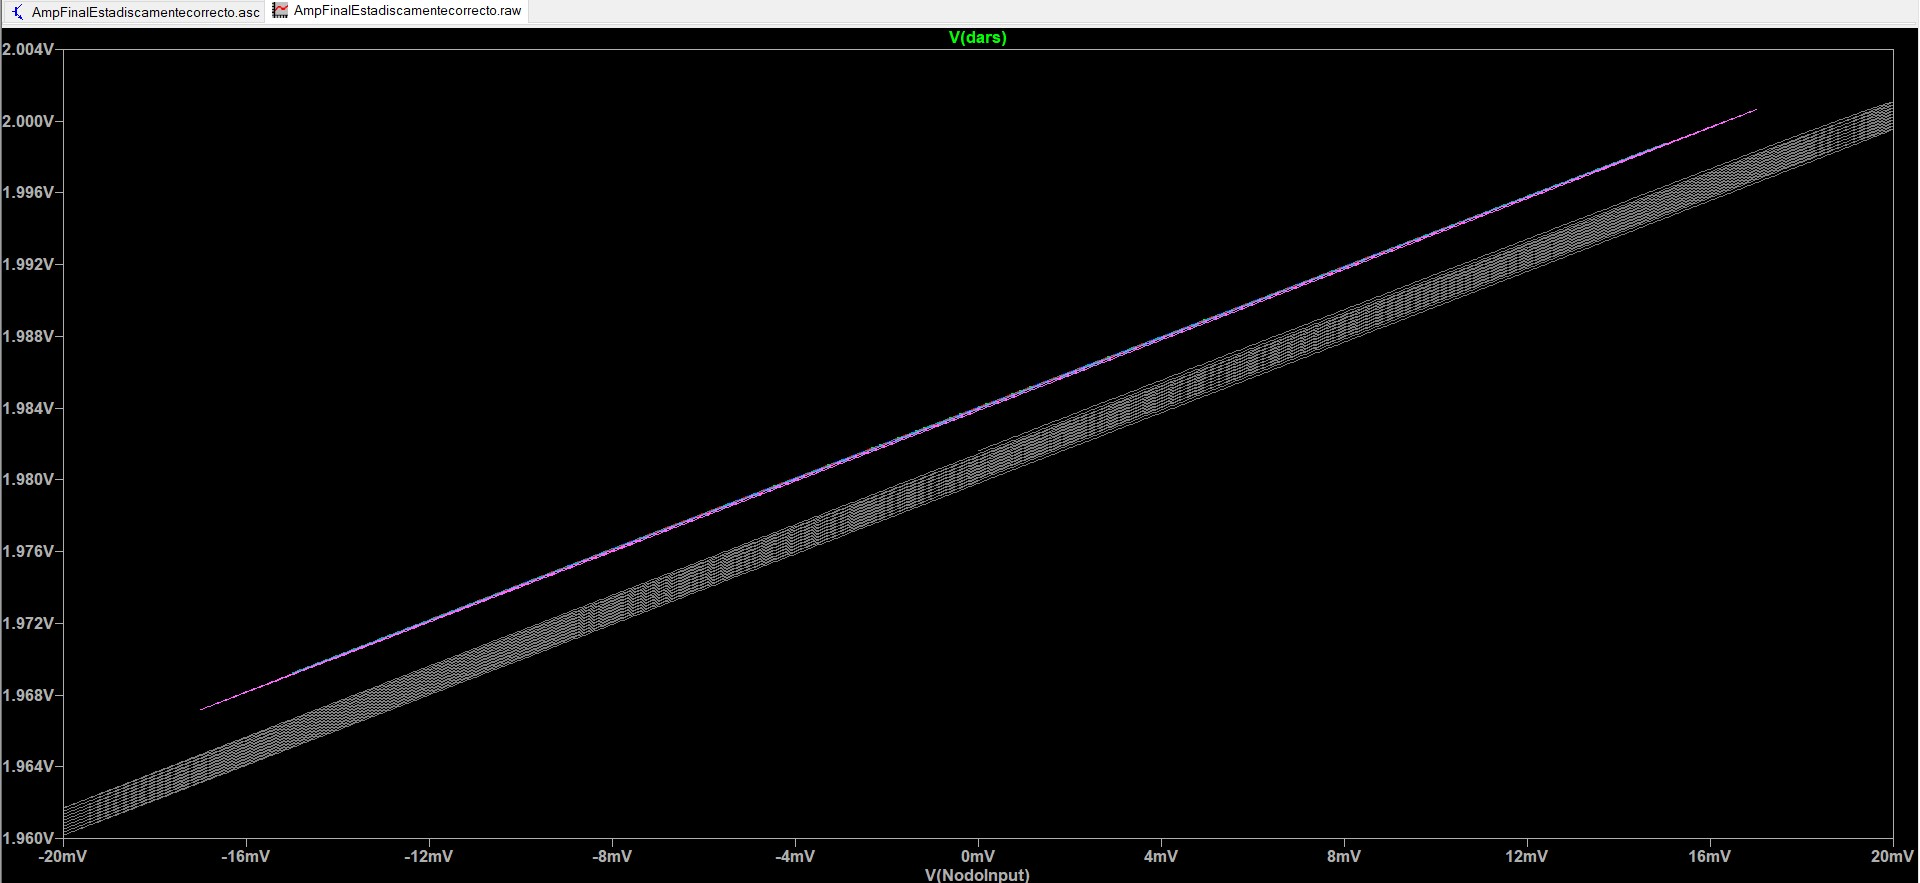
\includegraphics[width=\linewidth]{Simu/LINEALIDAD-DAR.jpg}
        \caption{Evaluación de Linealidad.}
      \label{SimuLinDar}
    \end{minipage}
\end{figure}

% =========================================================================
% APARTADO 3: ETAPA EMISOR COMUN
% =========================================================================

\subsubsection{Segunda Etapa: Ganancia de Tensión en Emisor Común ($Q_3$)}
%\section{3. Segunda Etapa: Ganancia de Tensión en Emisor Común ($Q_3$)}

\begin{figure}[H]
    \centering
    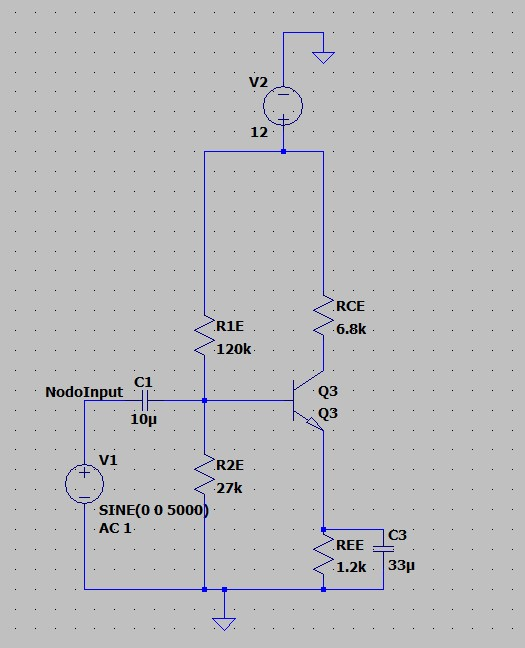
\includegraphics[width=0.45\linewidth]{Simu/Emisor_Aislado.jpg}
    \caption{Circuito esquemático de la etapa de Emisor Común aislada.}
\end{figure}

\vspace{0.5em}
{\small\textbf{Polarización y Disipación de Potencia}}

%\subsubsection{3.1. Polarización y Disipación de Potencia}
Se utilizó la directiva \texttt{.op} para registrar la corriente de colector $I_{C3}$ y la tensión $V_{CE3}$, asegurando la ubicación del punto de trabajo en la región activa.
\begin{verbatim}
.op
.meas DC VCE_Q3 PARAM V(NodoColector_Q3)-V(NodoEmisor_Q3)
.meas DC IC_Q3 I(Q3)
\end{verbatim}

\vspace{0.5em}
{\small\textbf{Medición de Impedancias de la Etapa Emisor Común ($Z_{in2}$ y $Z_{out2}$)}}

%\subsubsection{3.2. Medición de Impedancias de la Etapa Emisor Común ($Z_{in2}$ y $Z_{out2}$)}
Para la impedancia de entrada $Z_{in2}$, se aplicó tensión en la base de $Q_3$. Para la impedancia de salida $Z_{out2}$, se desacopló la carga/tercera etapa, se pasivó la entrada y se aplicó una fuente de prueba en el colector.

\paragraph{Impedancia de Entrada ($Z_{in2}$)}
Se puede ver en (\cref{SimuZin2}).
\begin{figure}[H]
    \centering
    \begin{minipage}{0.48\textwidth}
        \centering
        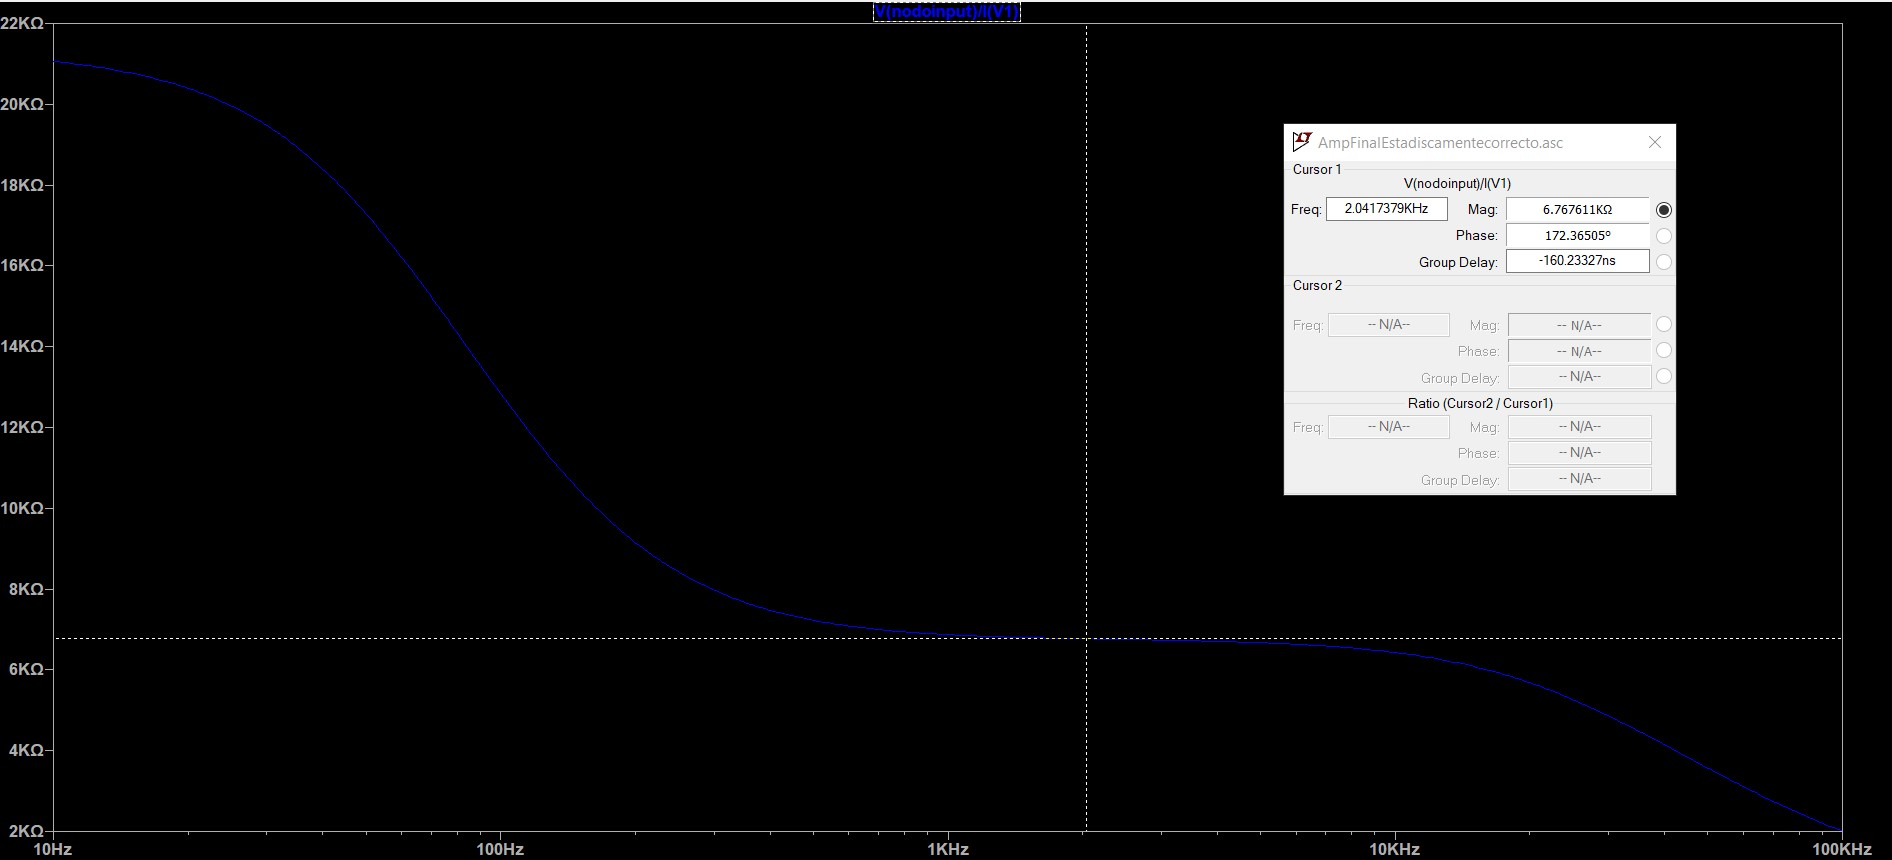
\includegraphics[width=\linewidth]{Simu/Emisor_ZIN.jpg}
        \caption{Curva de respuesta de $Z_{in2}$.}
      \label{SimuZin2}
    \end{minipage}
\end{figure}

\paragraph{Impedancia de Salida ($Z_{out2}$)}
Se puede ver en (\cref{SimuZout2}).
\begin{figure}[H]
    \centering
    \begin{minipage}{0.48\textwidth}
        \centering
        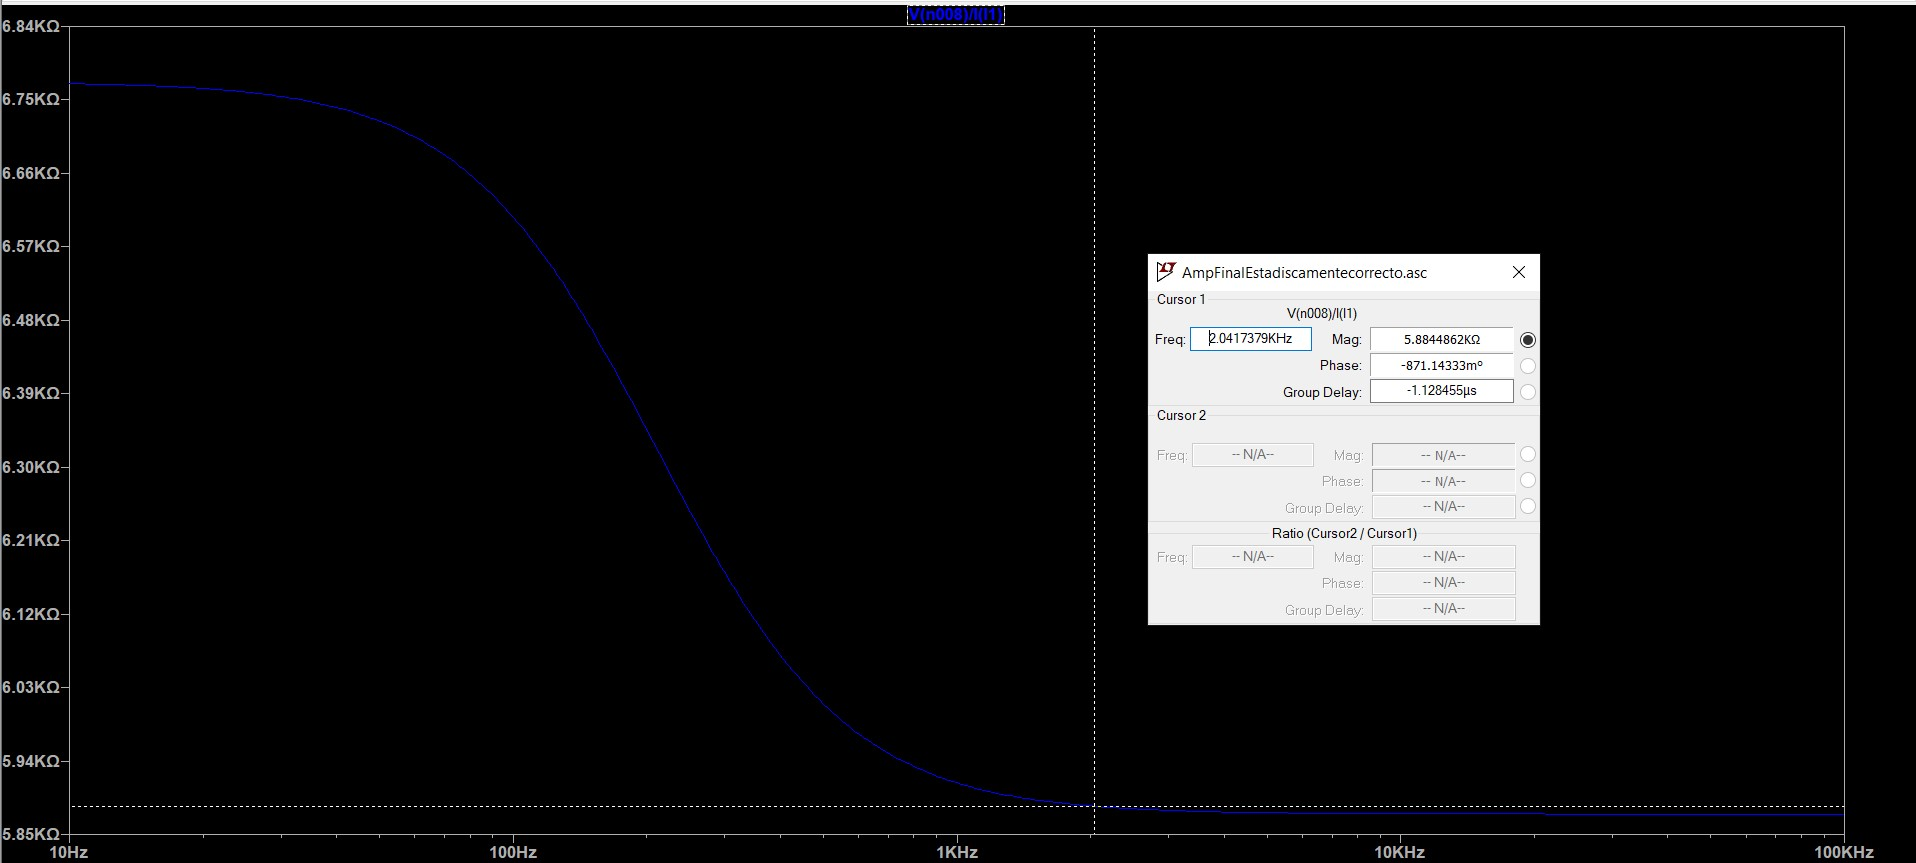
\includegraphics[width=\linewidth]{Simu/Emisor_Zout.jpg}
        \caption{Curva de respuesta de $Z_{out2}$.}
      \label{SimuZout2}
    \end{minipage}
\end{figure}

\vspace{0.5em}
{\small\textbf{Respuesta en Frecuencia, Temporal, Ruido, Límites de $V_{CC}$ y Linealidad}}

%\subsubsection{3.3. Respuesta en Frecuencia, Temporal, Ruido, Límites de $V_{CC}$ y Linealidad}
Se analizó la ganancia de tensión y respuesta frecuencial (\texttt{.ac}), la respuesta temporal (\texttt{.tran}), la PSD de ruido (\texttt{.noise}), el límite por variación de la fuente $V_{CC}$ y la pérdida de linealidad mediante la transferencia $V_{out}$ vs $V_{in}$ (\cref{SimuBWEC}, \cref{SimuETEC}, \cref{SimuPSDEC}, \cref{SimuVarVccEC}, \cref{SimuLinEC}).

\begin{figure}[H]
    \centering
    \begin{minipage}{0.48\textwidth}
        \centering
        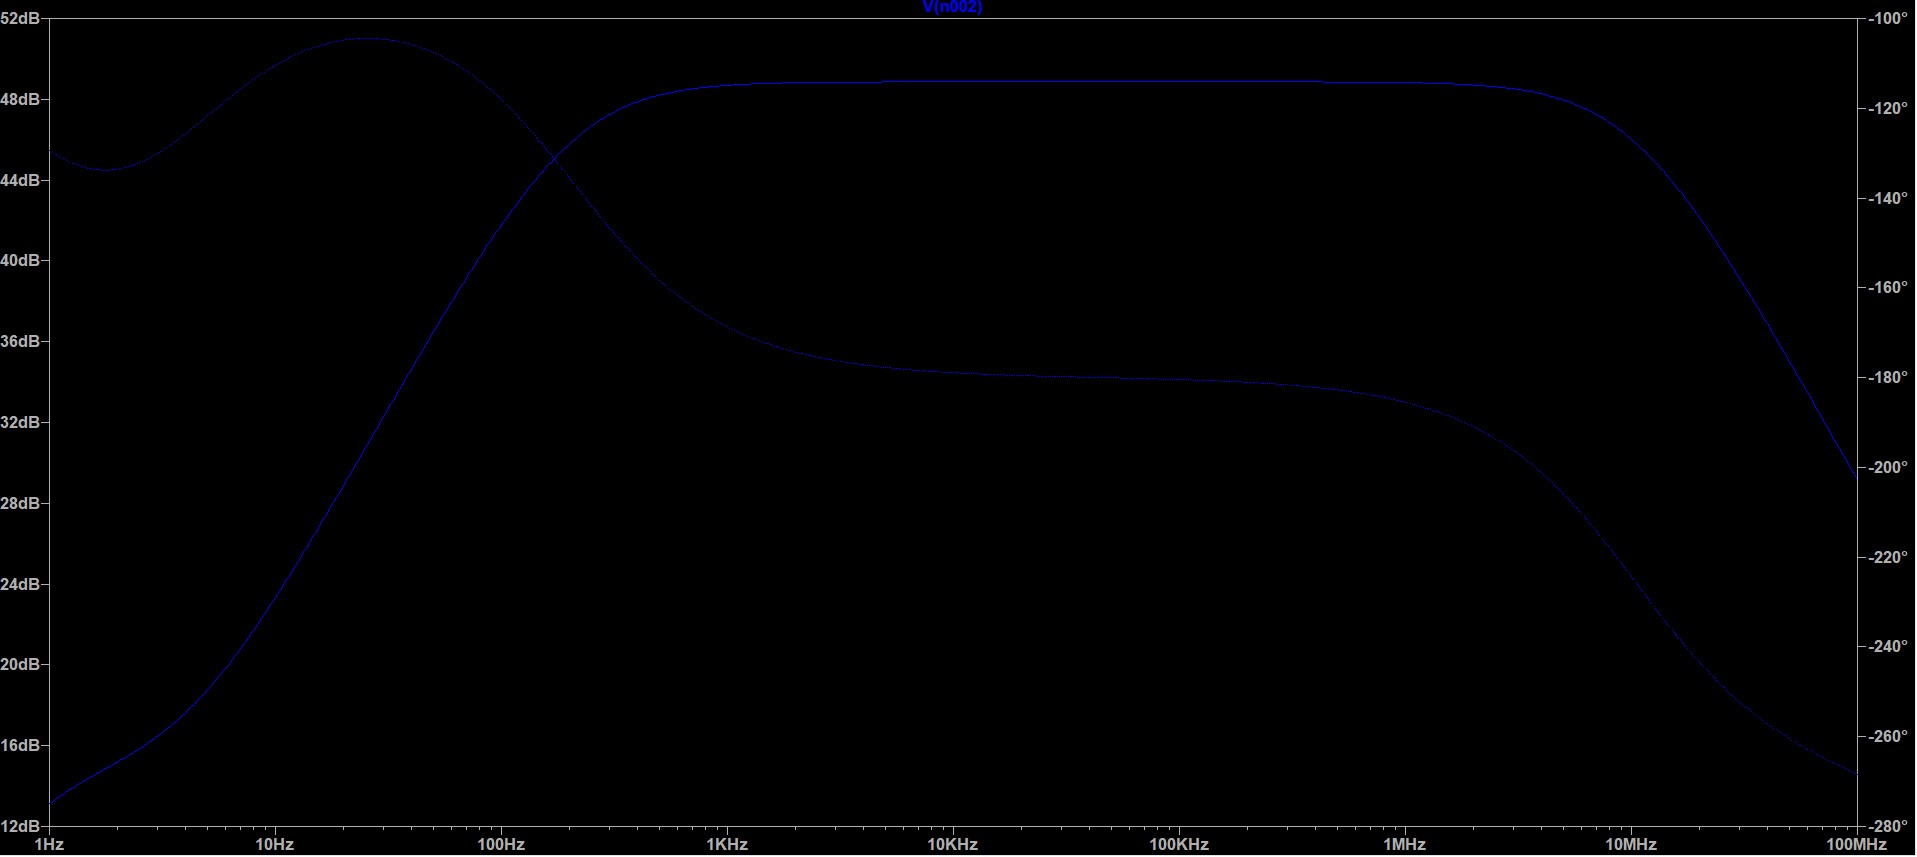
\includegraphics[width=\linewidth]{Simu/BW-EMISOR.jpg}
        \caption{Ancho de banda - Emisor Común.}
      \label{SimuBWEC}
    \end{minipage}\hfill
    \begin{minipage}{0.48\textwidth}
        \centering
        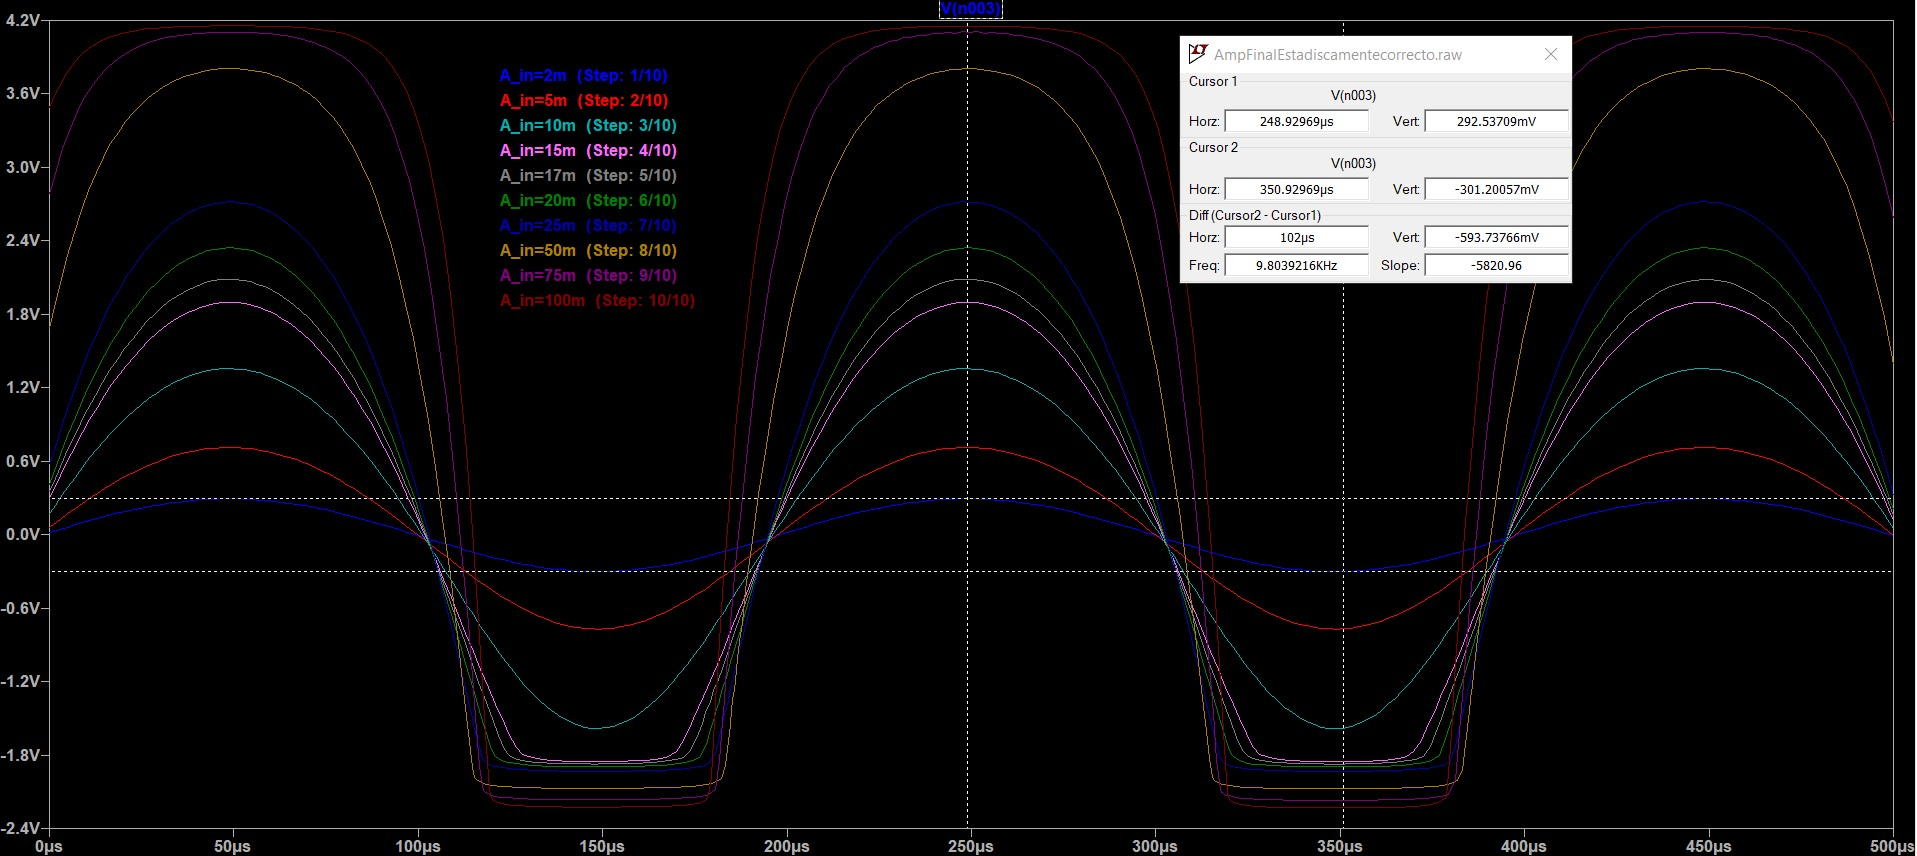
\includegraphics[width=\linewidth]{Simu/VPP-EMISOR.jpg}
        \caption{Excursión temporal $V_{pp}$.}
      \label{SimuETEC}
    \end{minipage}
\end{figure}

\begin{figure}[H]
    \centering
    \begin{minipage}{0.48\textwidth}
        \centering
        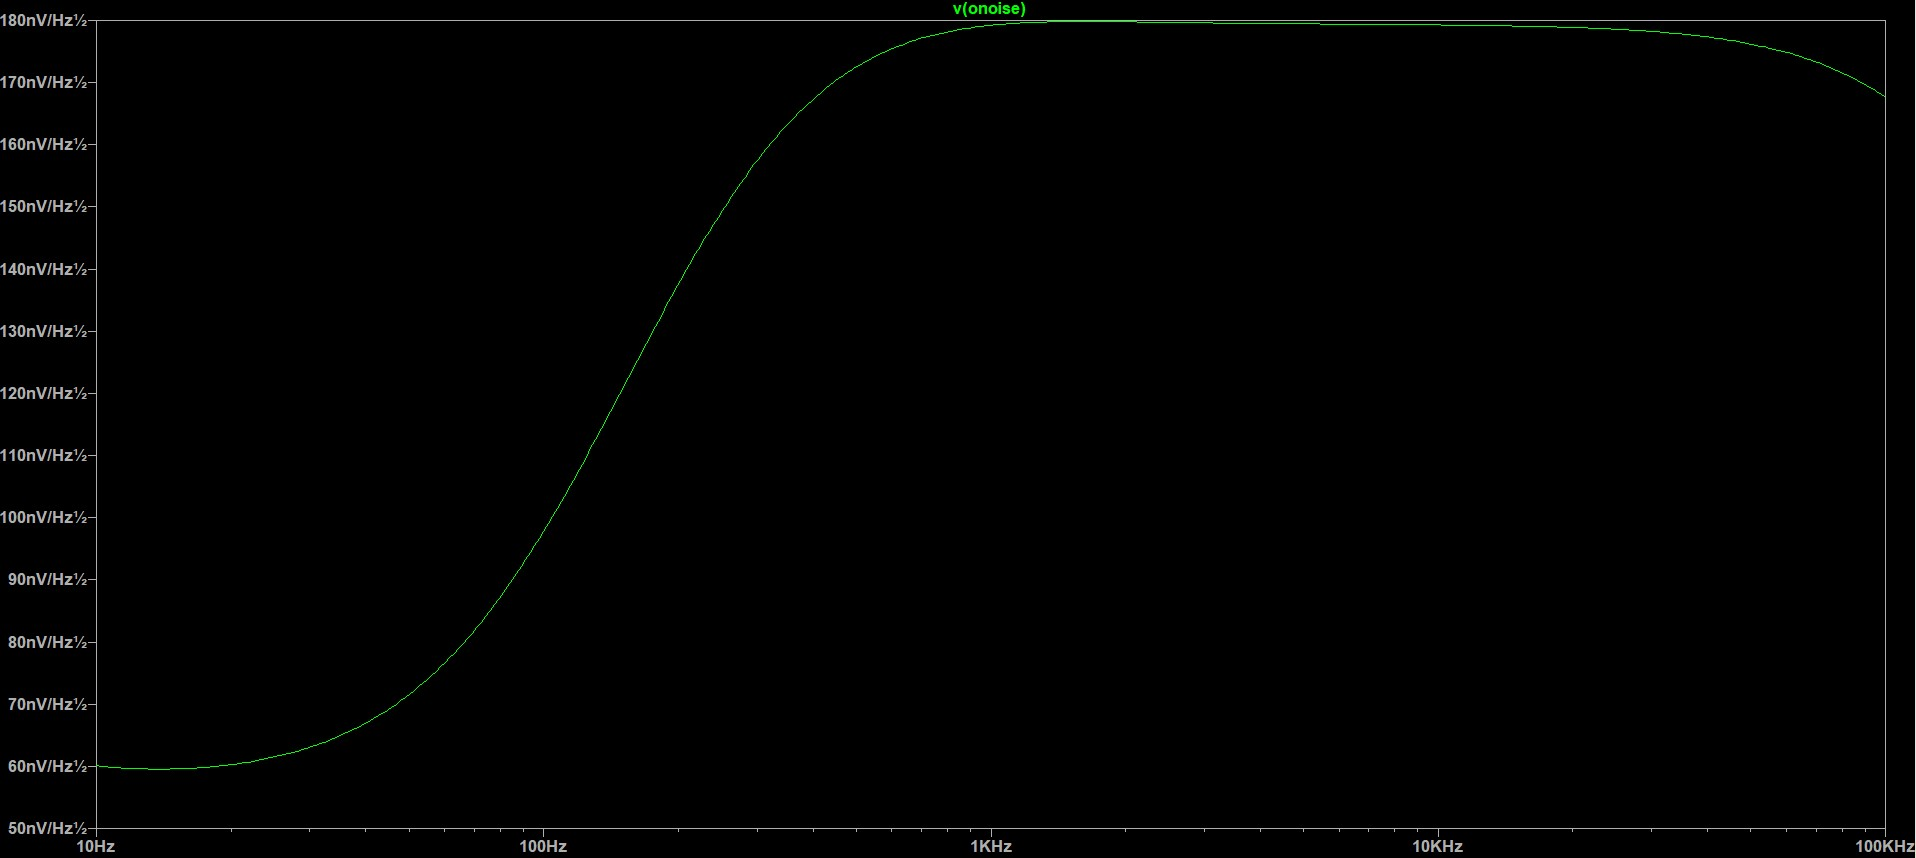
\includegraphics[width=\linewidth]{Simu/NOISE-EM.jpg}
        \caption{PSD de Ruido - Emisor Común.}
      \label{SimuPSDEC}
    \end{minipage}\hfill
    \begin{minipage}{0.48\textwidth}
        \centering
        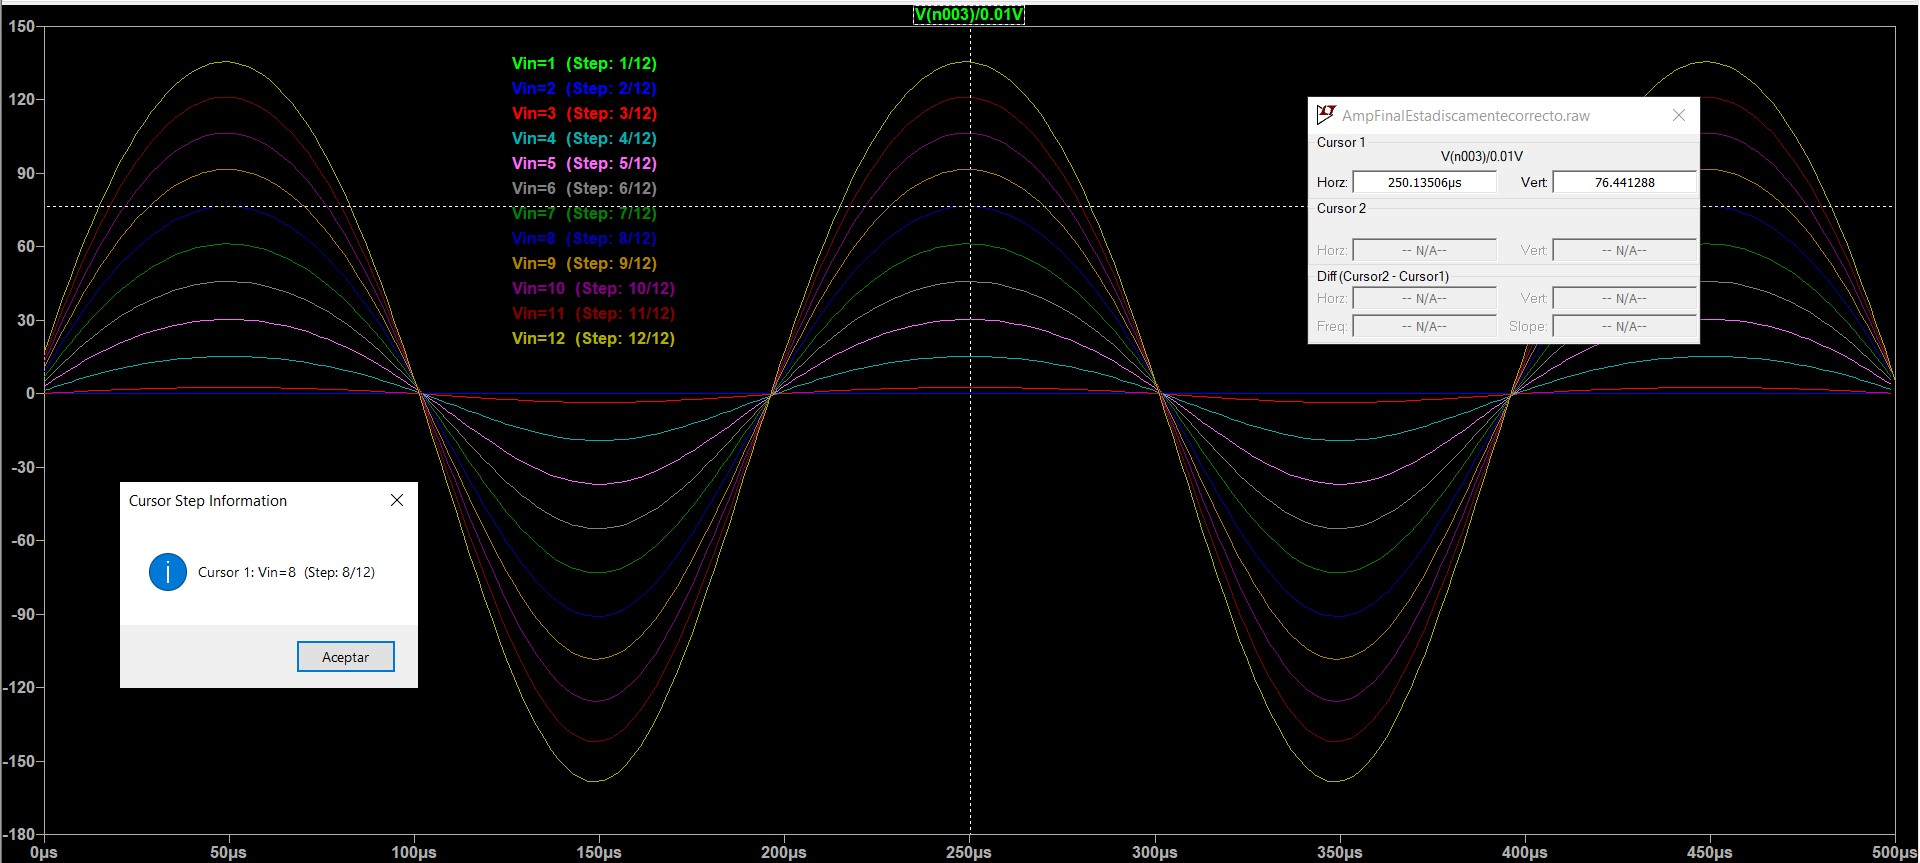
\includegraphics[width=\linewidth]{Simu/VCC-EMISOR.jpg}
        \caption{Variación de la fuente $V_{CC}$.}
      \label{SimuVarVccEC}
    \end{minipage}
\end{figure}

\begin{figure}[H]
    \centering
    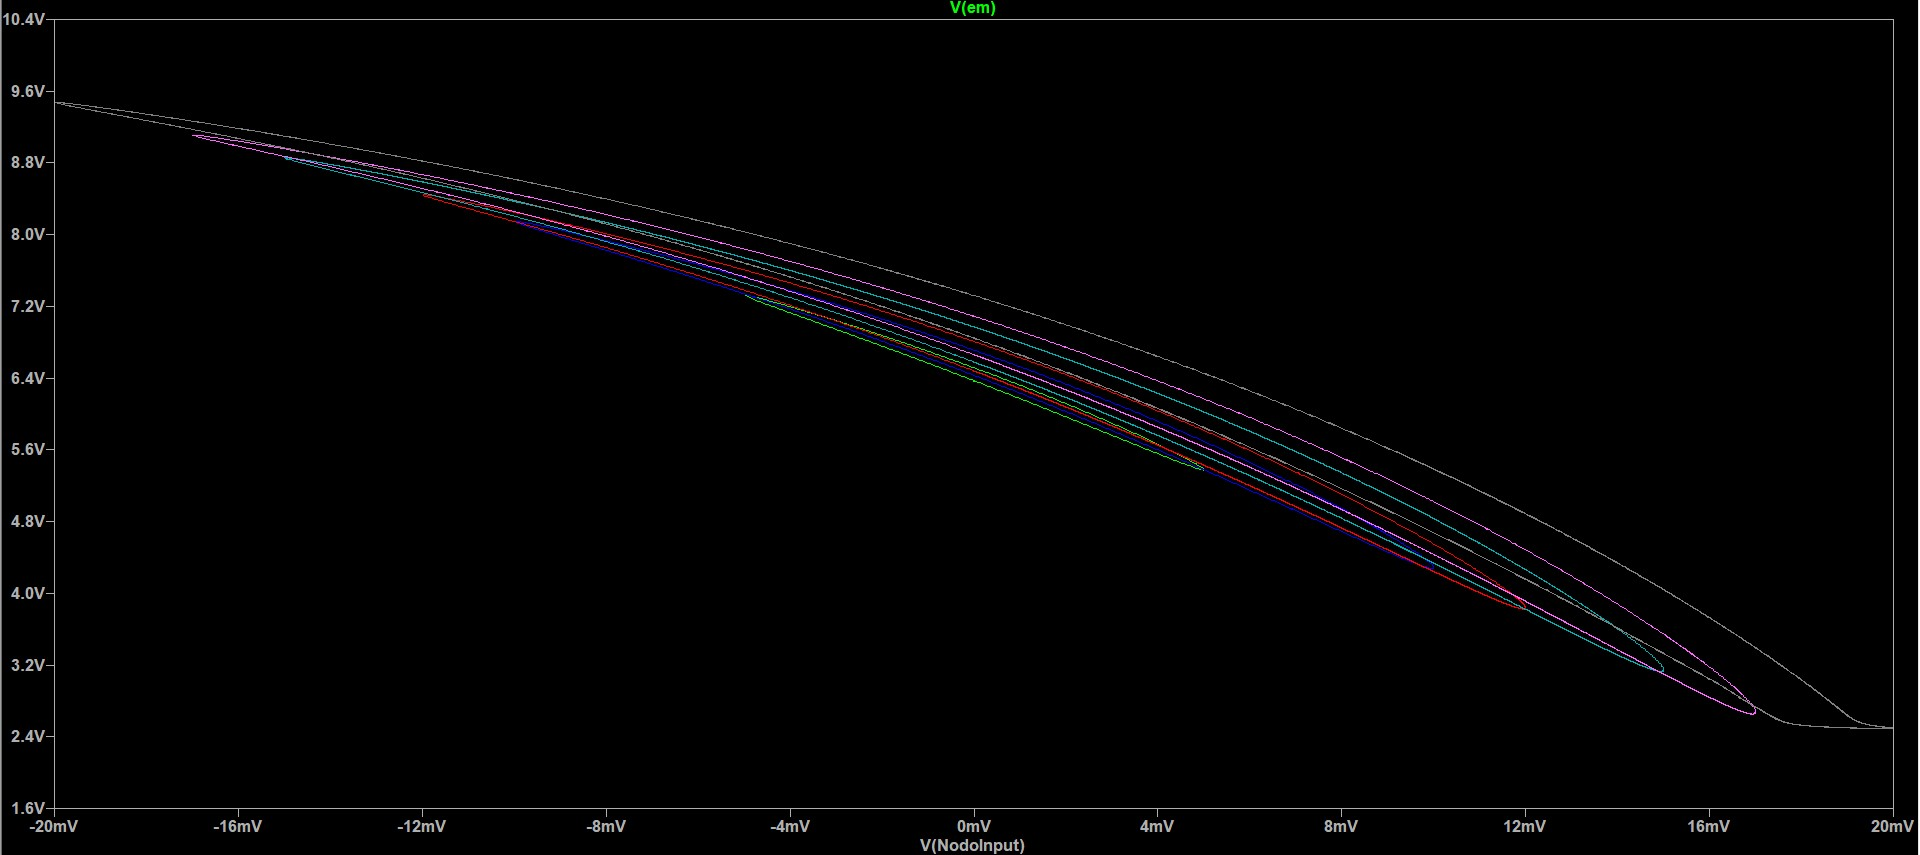
\includegraphics[width=0.75\linewidth]{Simu/Linealidad-em.jpg}
    \caption{Límites de linealidad de la etapa en Emisor Común.}
  \label{SimuLinEC}
\end{figure}
% =========================================================================
% APARTADO 4: ETAPA SZIKLAI
% =========================================================================
\subsubsection{Tercera Etapa: Salida Sziklai ($Q_4$ - $Q_5$)}
%\section{4. Tercera Etapa: Salida Sziklai ($Q_4$ - $Q_5$)}

\begin{figure}[H]
    \centering
    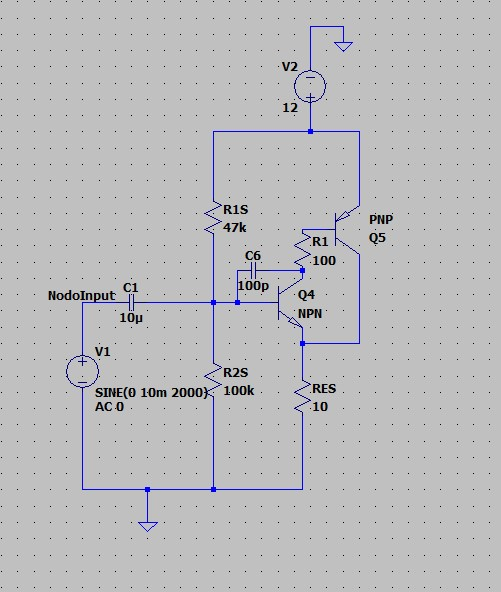
\includegraphics[width=0.45\linewidth]{Simu/sql-aislado.jpg}
    \caption{Circuito esquemático de la etapa de potencia Sziklai aislada.}
\end{figure}

\vspace{0.5em}
{\small\textbf{Polarización y Disipación de Potencia}}

%\subsubsection{4.1. Polarización y Disipación de Potencia}
Mediante \texttt{.op} se verificó la corriente de reposo que circula por los transistores $Q_4$ y $Q_5$ para confirmar la eliminación de la distorsión por cruce por cero (crossover).
\begin{verbatim}
.op
.meas DC I_Q4 I(Q4)
.meas DC I_Q5 I(Q5)
\end{verbatim}

\vspace{0.5em}
{\small\textbf{Medición de Impedancias de la Etapa Sziklai ($Z_{in3}$ y $Z_{out3}$)}}

%\subsubsection{4.2. Medición de Impedancias de la Etapa Sziklai ($Z_{in3}$ y $Z_{out3}$)}
Se determinó la impedancia de entrada vista desde la base de $Q_4$ y la impedancia de salida que presenta el par Sziklai hacia la carga de $8\,\Omega$.

\paragraph{Impedancia de Entrada ($Z_{in3}$)}
Se puede ver en (\cref{SimuZin3}).
\begin{figure}[H]
    \centering
    \begin{minipage}{0.48\textwidth}
        \centering
        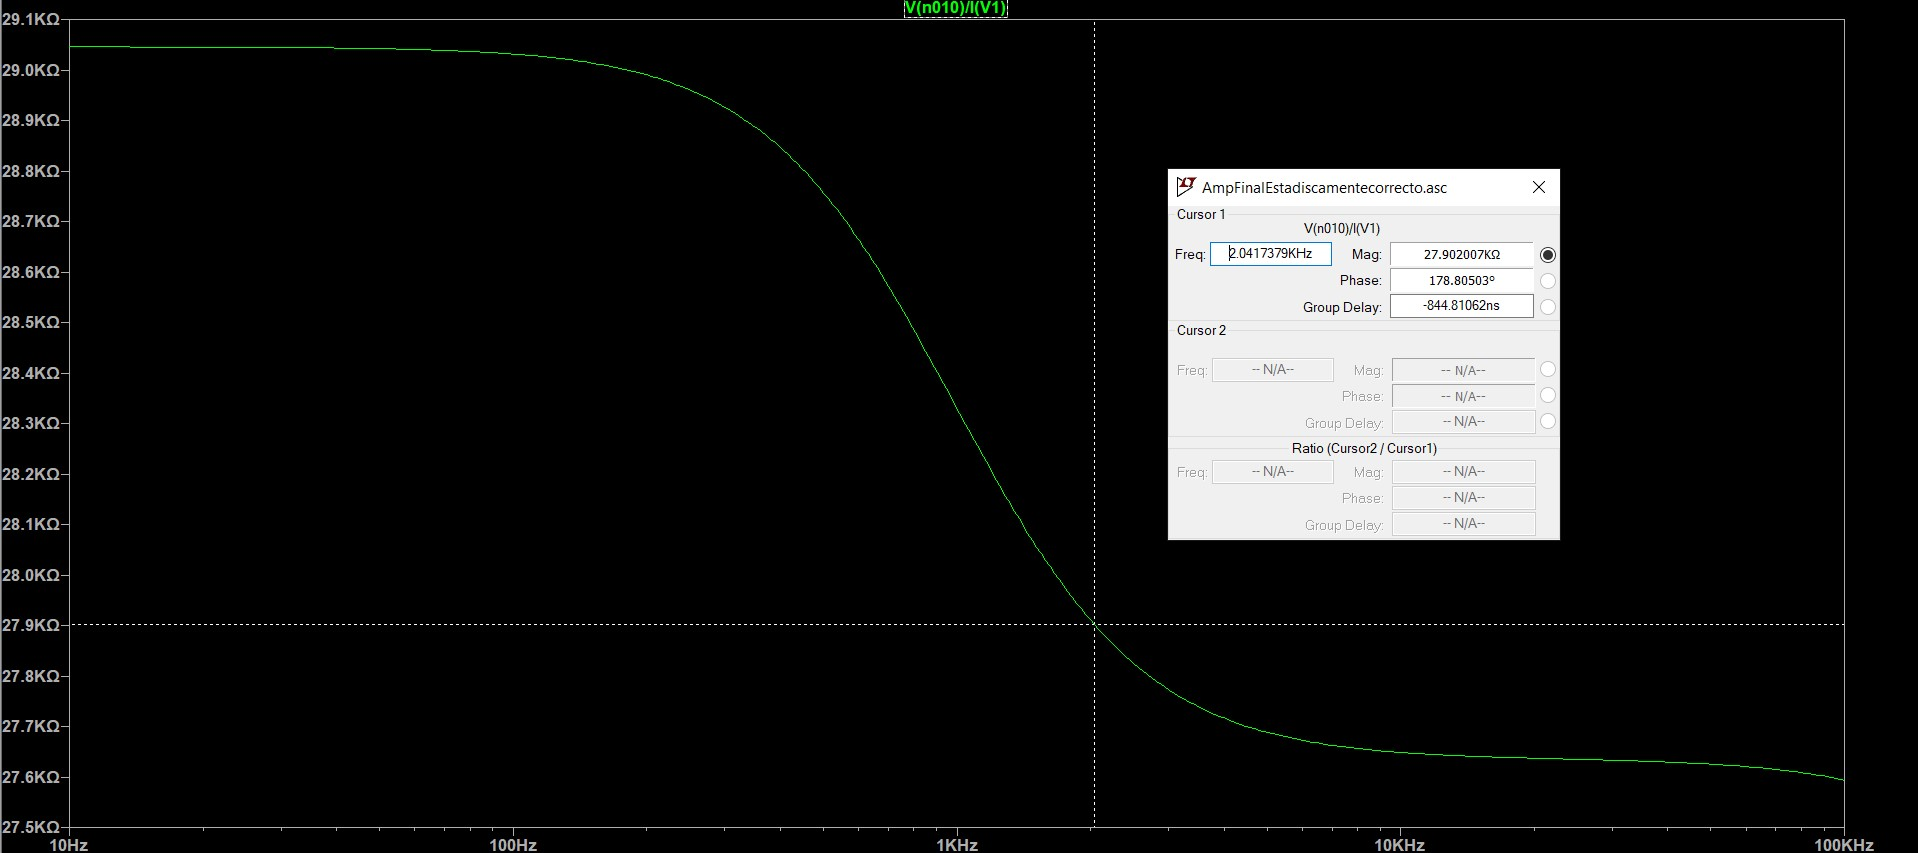
\includegraphics[width=\linewidth]{Simu/SQL_ZIN.jpg}
        \caption{Curva de respuesta de $Z_{in3}$.}
      \label{SimuZin3}
    \end{minipage}
\end{figure}

\paragraph{Impedancia de Salida ($Z_{out3}$)}
Se puede ver en (\cref{SimuZout3}).
\begin{figure}[H]
    \centering
    \begin{minipage}{0.48\textwidth}
        \centering
        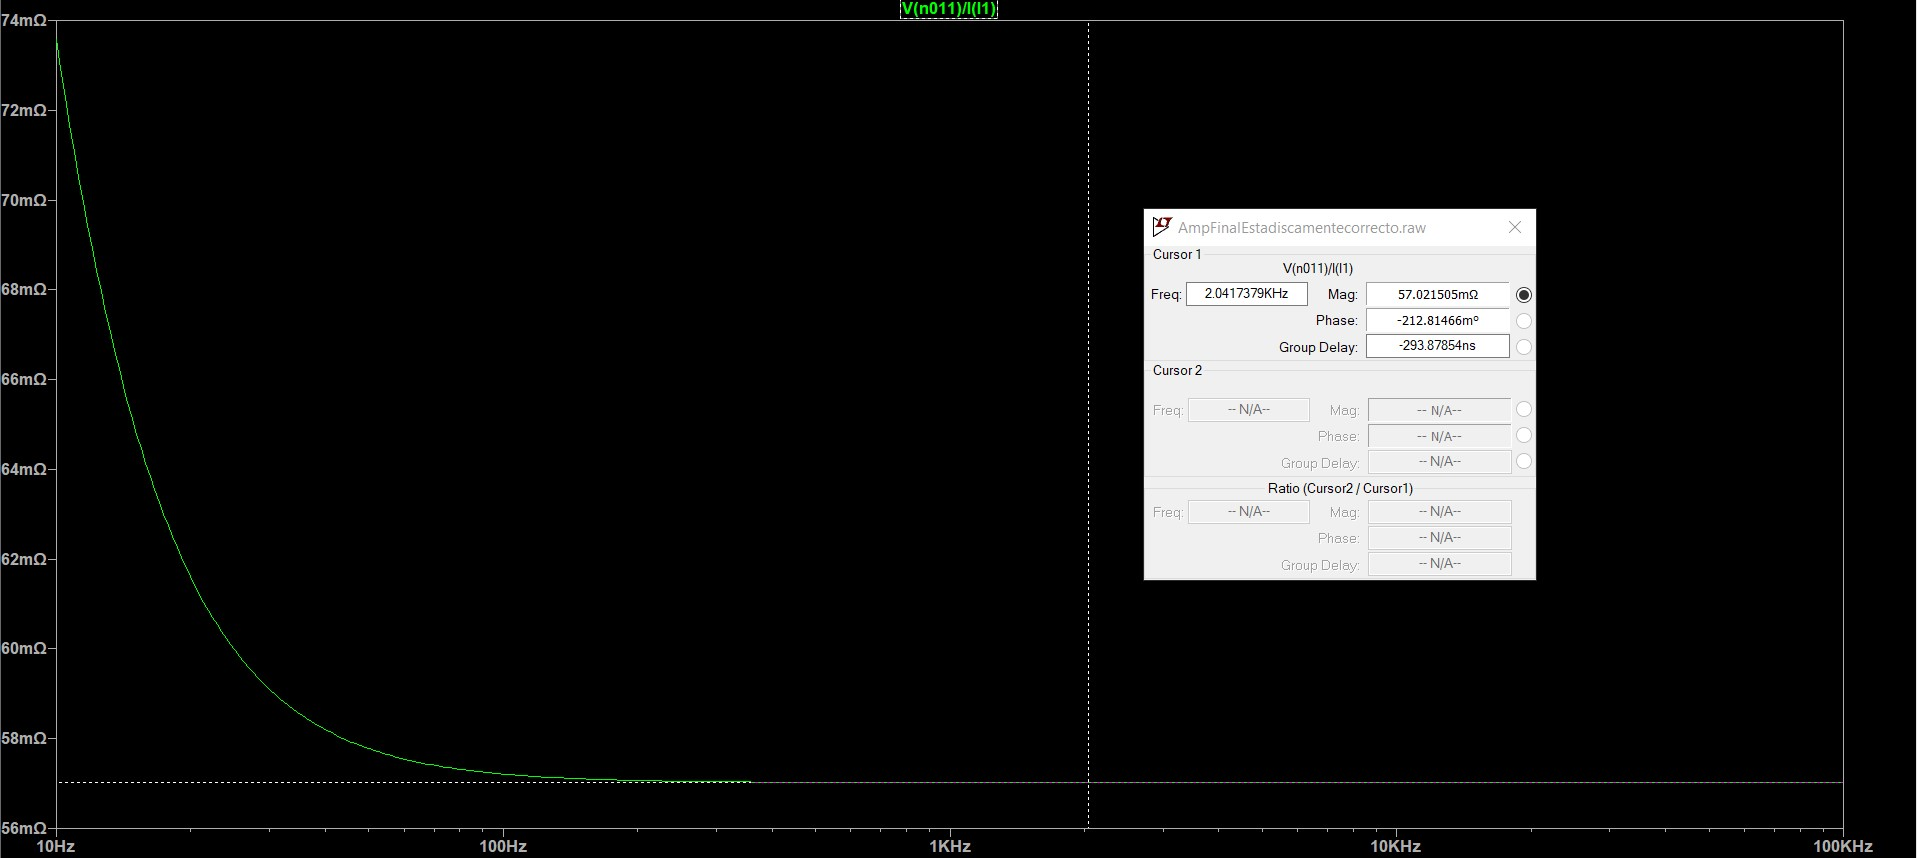
\includegraphics[width=\linewidth]{Simu/SQL_ZOUT.jpg}
        \caption{Curva de respuesta de $Z_{out3}$.}
      \label{SimuZout3}
    \end{minipage}
\end{figure}

\vspace{0.5em}
{\small\textbf{Respuesta en Frecuencia, Temporal, Ruido, Límites de $V_{CC}$ y Linealidad)}}

%\subsubsection{4.3. Respuesta en Frecuencia, Temporal, Ruido, Límites de $V_{CC}$ y Linealidad}
  Se evaluó el comportamiento de la etapa Sziklai en régimen dinámico, registrando el ancho de banda (\texttt{.ac}), la respuesta temporal (\texttt{.tran}), el ruido (\texttt{.noise}), la tolerancia ante variaciones de la fuente $V_{CC}$ y el límite de linealidad antes del recorte (\cref{SimuBWSz}, \cref{SimuTepSz}, \cref{SimuPSDSz}, \cref{SimuVarVccSz}, \cref{SimuLinSz}).

\begin{figure}[H]
    \centering
    \begin{minipage}{0.48\textwidth}
        \centering
        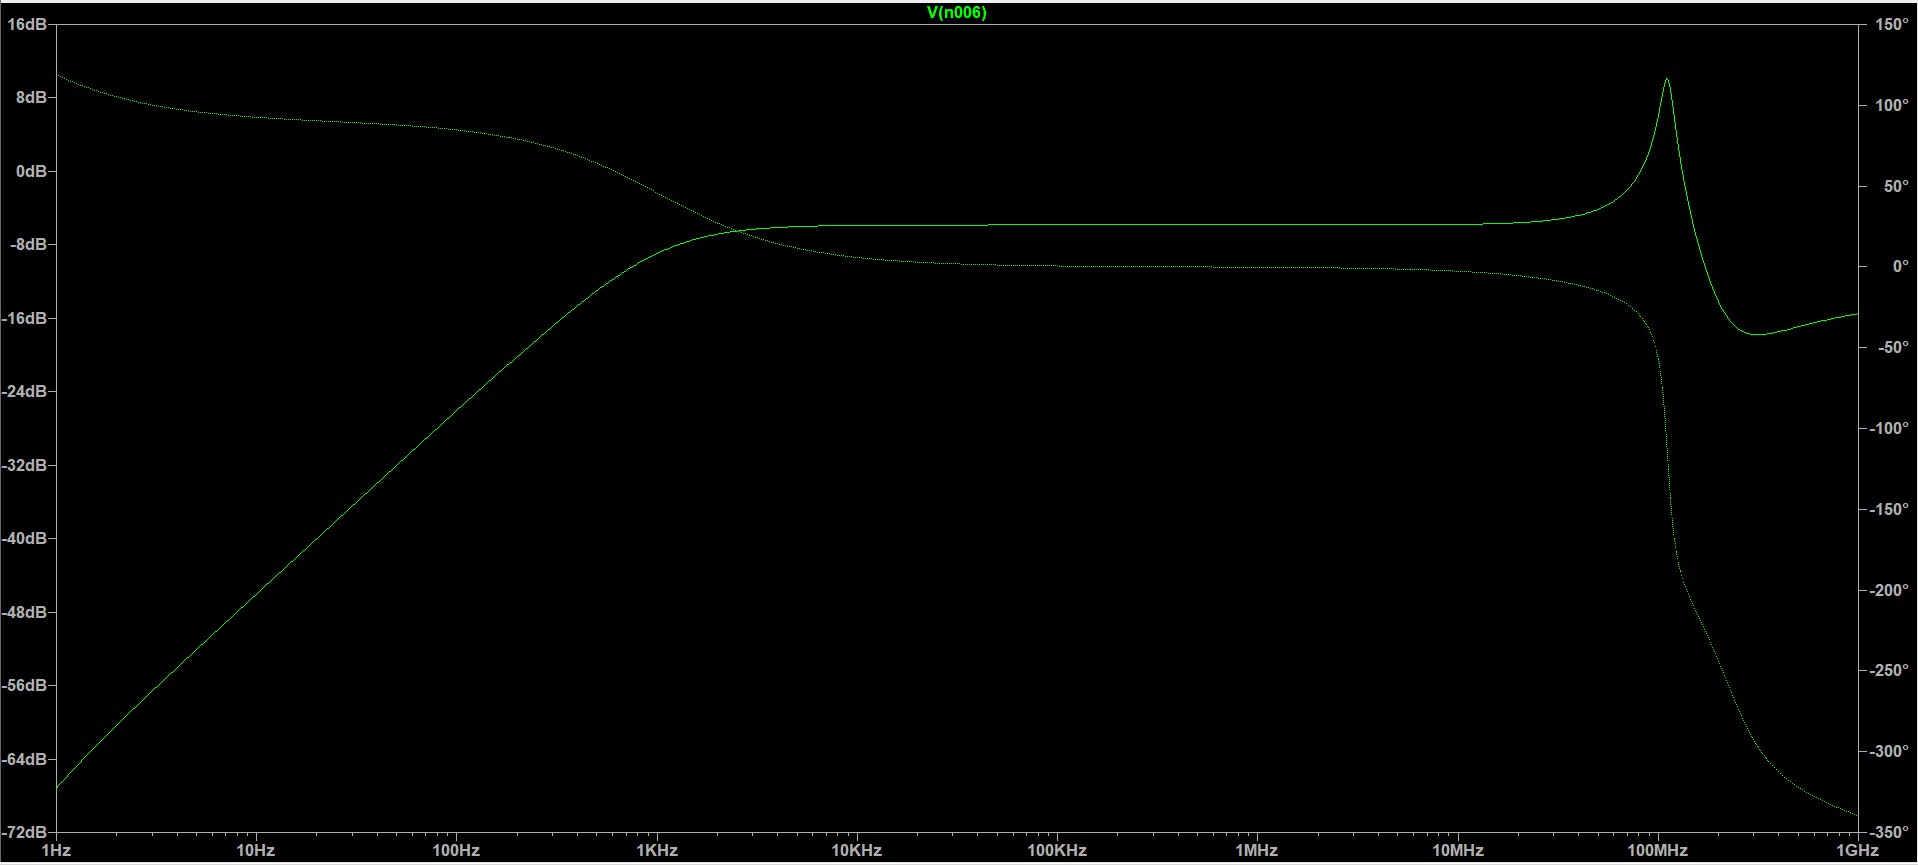
\includegraphics[width=\linewidth]{Simu/BW-SQL.jpg}
        \caption{Ancho de banda - Etapa Sziklai.}
      \label{SimuBWSz}
    \end{minipage}\hfill
    \begin{minipage}{0.48\textwidth}
        \centering
        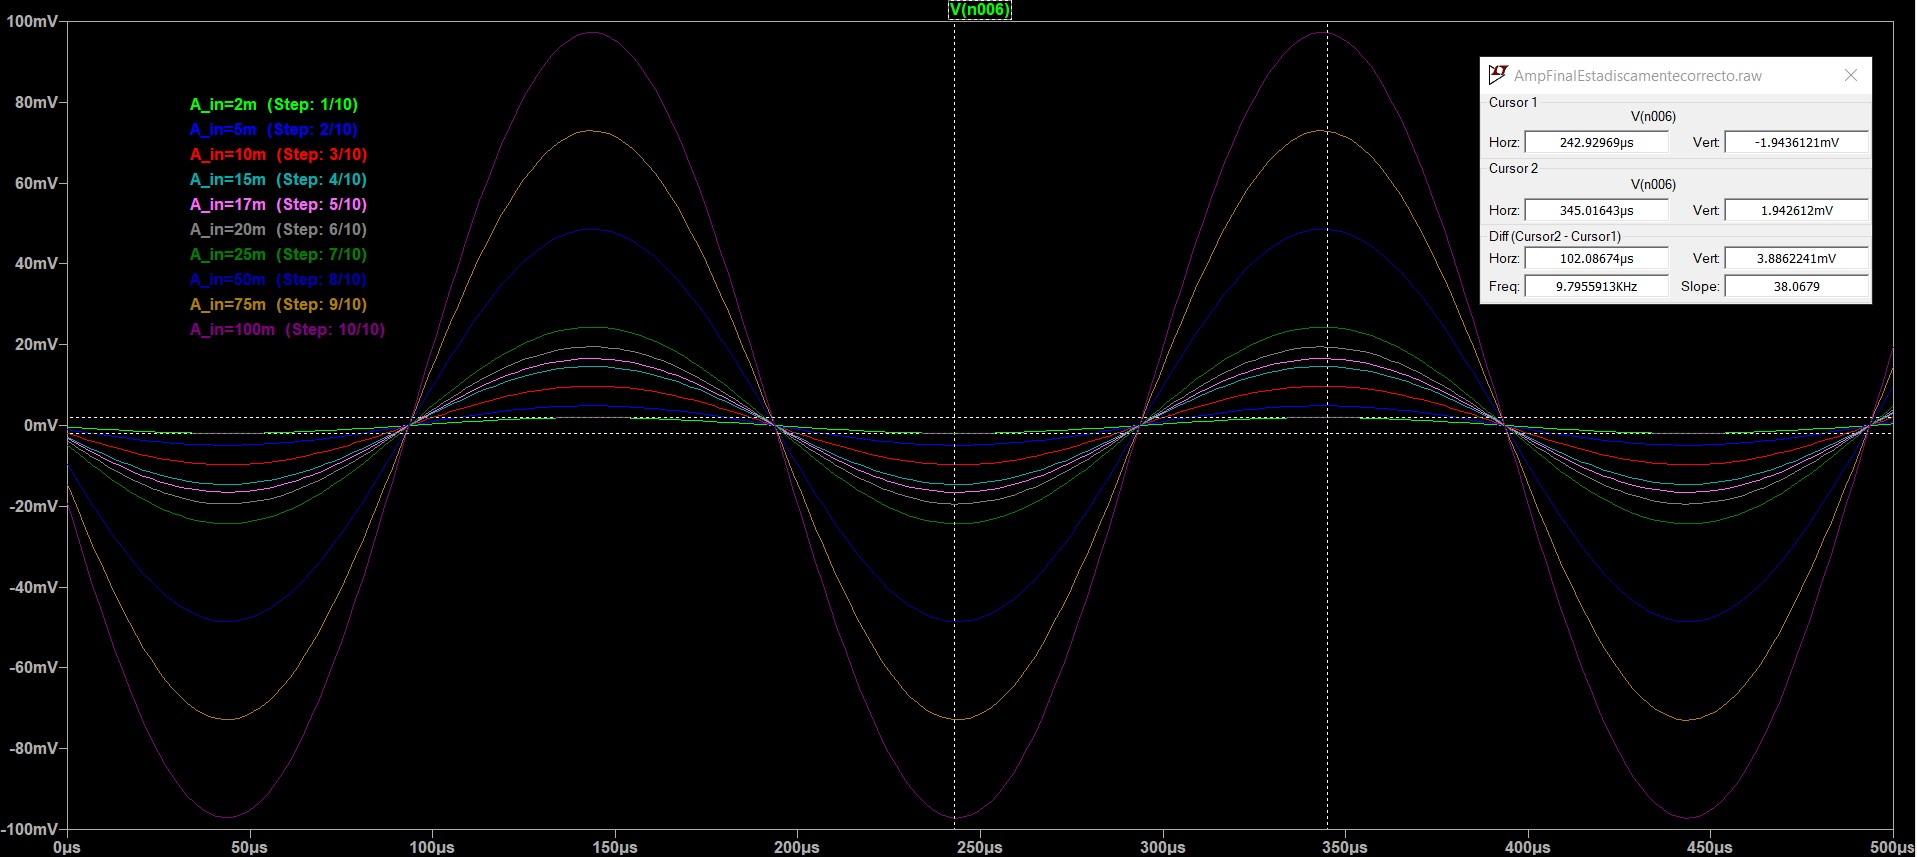
\includegraphics[width=\linewidth]{Simu/VPP-SQL.jpg}
        \caption{Respuesta temporal en la carga.}
      \label{SimuTepSz}
    \end{minipage}
\end{figure}

\begin{figure}[H]
    \centering
    \begin{minipage}{0.48\textwidth}
        \centering
        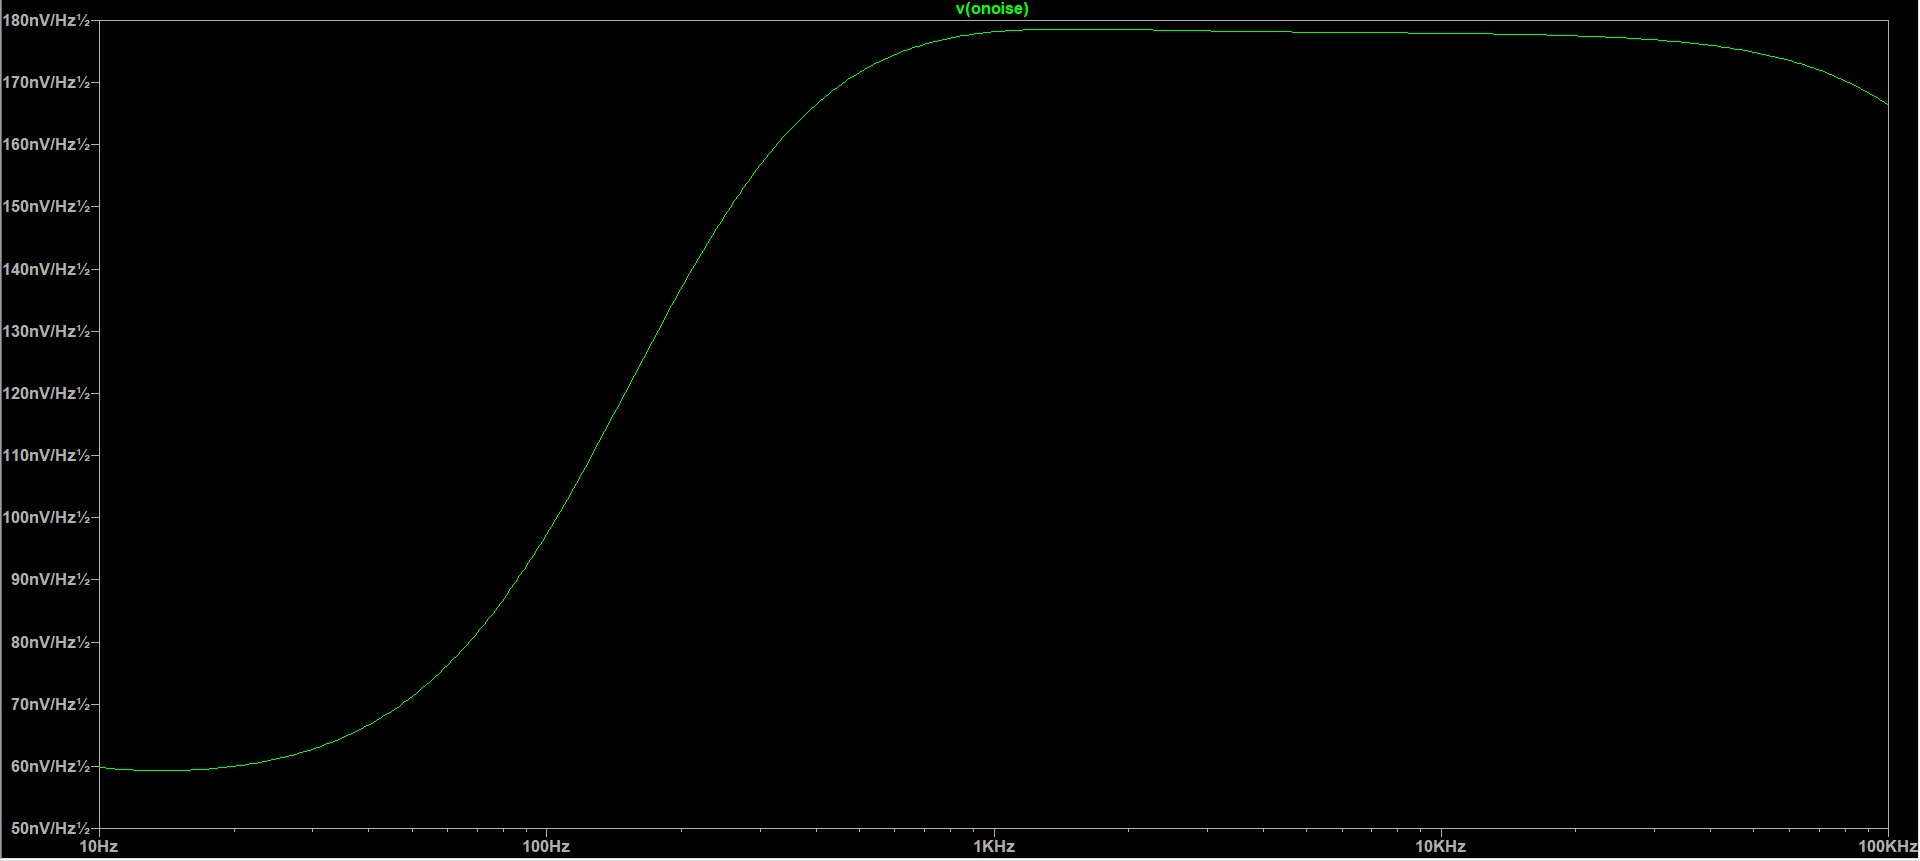
\includegraphics[width=\linewidth]{Simu/NOISE-SQL.jpg}
        \caption{PSD de Ruido - Etapa Sziklai.}
      \label{SimuPSDSz}
    \end{minipage}\hfill
    \begin{minipage}{0.48\textwidth}
        \centering
        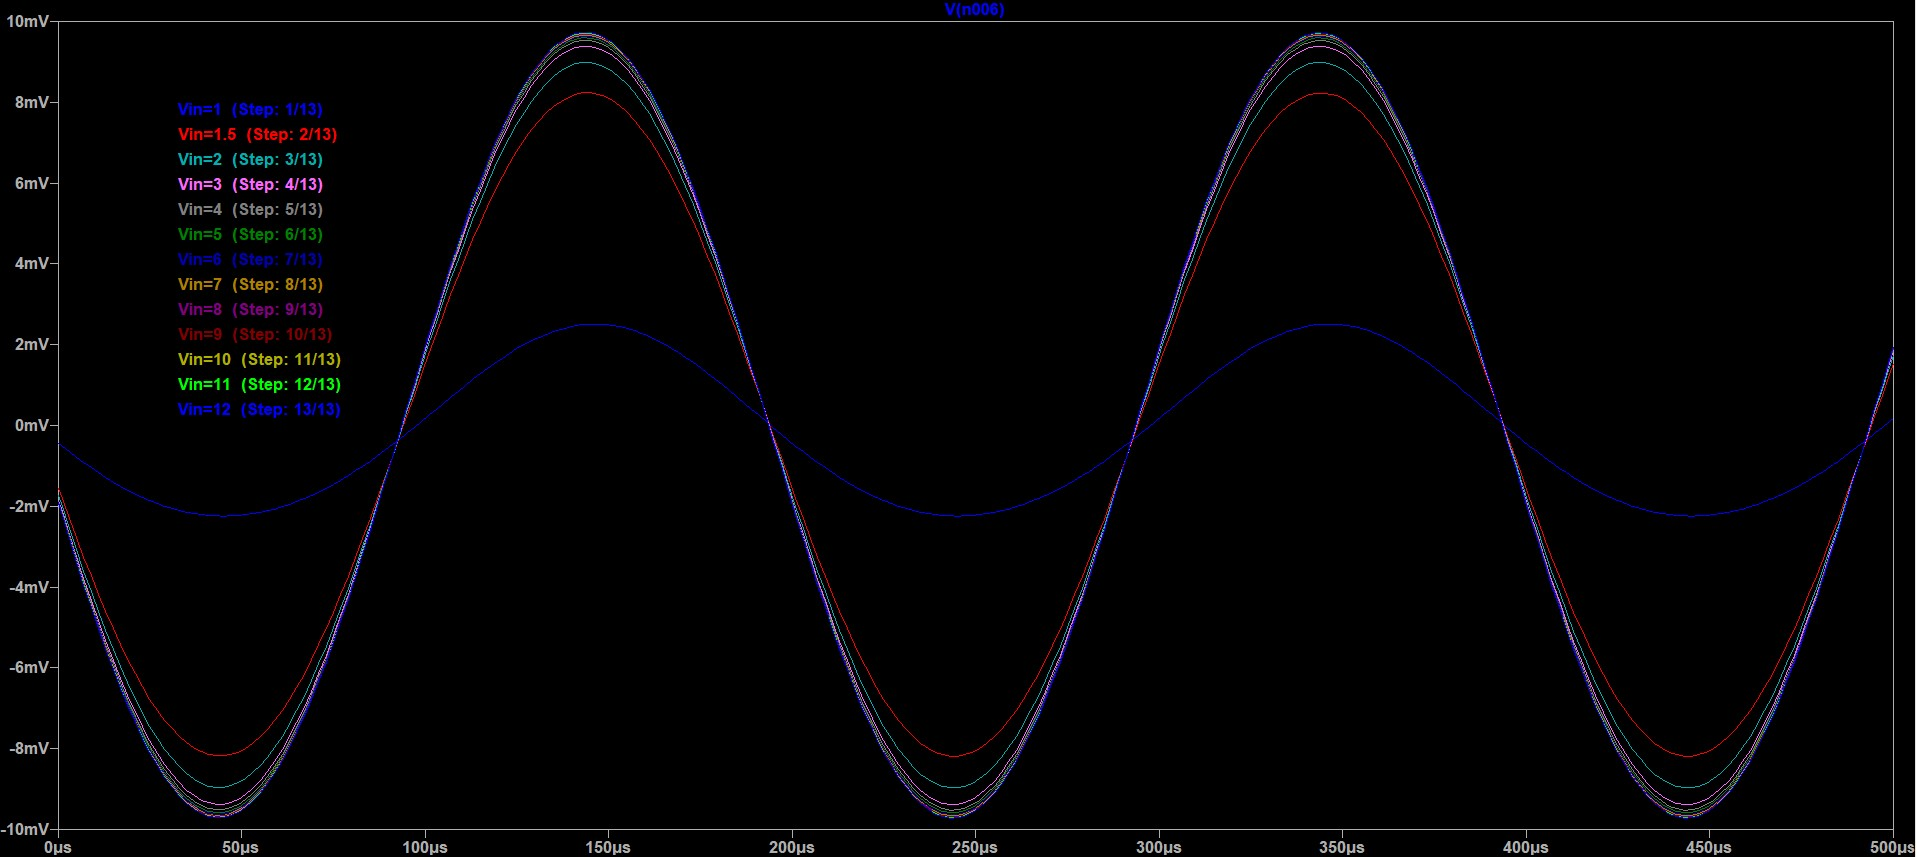
\includegraphics[width=\linewidth]{Simu/vcc-sql.jpg}
        \caption{Variación de la fuente $V_{CC}$.}
      \label{SimuVarVccSz}
    \end{minipage}
\end{figure}

\begin{figure}[H]
    \centering
    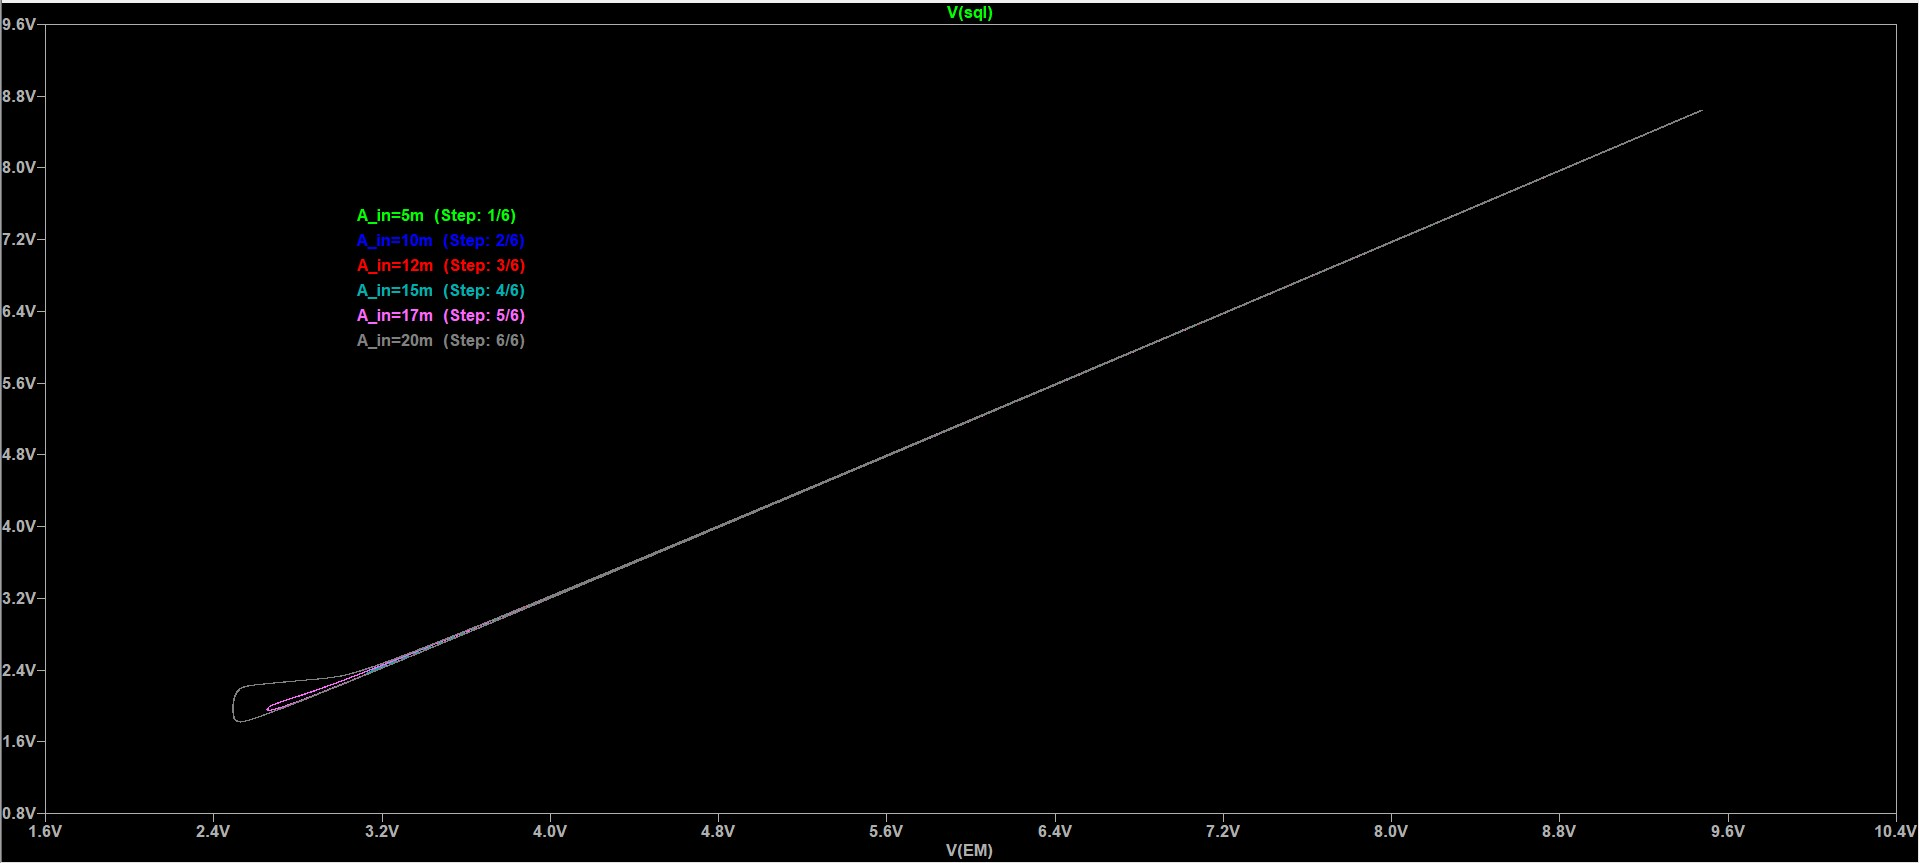
\includegraphics[width=0.75\linewidth]{Simu/Linealidad-sql.jpg}
    \caption{Límites de linealidad de la etapa Sziklai observando la salida.}
  \label{SimuLinSz}
\end{figure}

% =========================================================================
% APARTADO 5: NOTA ACLARATORIA SOBRE EL ALCANCE DE LAS SIMULACIONES
% =========================================================================

\subsubsection{Consideraciones sobre la Presentación y Documentación de los Resultados}
%\section{5. Consideraciones sobre la Presentación y Documentación de los Resultados}

Cabe destacar que la metodología analítica y los procedimientos de medición simulada expuestos de forma detallada en el análisis global (Sección 1) fueron aplicados de manera idéntica y sistemática pa cada una de las etapas del amplificador (Darlington, Emisor Común y Sziklai).

Con el objetivo de mantener la concisión, fluidez y claridad en la lecturao, la exposición gráfica en las Secciones 2, 3 y 4 se ha presentado de forma sintetizada, incorporando únicamente las figuras y curvas de respuesta consideradas más representativas para la comprensión del comportamiento de cada etapa aislada.

No obstante, la totalidad de los ensayos de simulación se encuentran  documentados y disponibles para su consulta y verificación en el repositorio de GitHub asociado a este trabajo práctico.
